\documentclass{article}
\usepackage{subfigure,graphicx}
\usepackage{amssymb}
\usepackage{float}

\title{Clustering of Time Series using Wavelet Transformations as a Feature Extraction Mechanism}
\author{\textsf{Josu\'e Kuri, Felix Huang, Ssurey Moon, Kathy Norman}\\UCSC Extension. 30164:(003) Machine Learning and Data Mining}

\begin{document}
\maketitle

\section{Introduction}
A time series is a sequence of data points indexed by time at regular intervals. This model is used to represent a wide range of metrics such as the daily closing price of stocks, temperature, precipitation, population, etc. In the context of machine learning and data mining, clustering of a large set of time series is an exploratory technique aimed at identifying and understanding underlying patterns.

Considering every point of a time series as a dimension results in a high dimensional space which clustering algorithms cannot handle easily. These algorithms depend on a distance measure as a basis to maximize cohesion and separation. In a high dimensional space, the contrast between the nearest and the farthest neighbor becomes smaller making it difficult for clustering algorithms to find meaninful groups \cite{BGRS99}.

Data dimensionality reduction is an approach to map a high dimensional space into a lower dimensional space such that the main characteristics of the data points in the original space are preserved and clustering on the lower dimensionality space results in meaningful groups. The two types of dimensionality reduction are feature selection and feature extraction. The former consists in selecting a subset of features from the original features. Feature extraction, on the other hand, generates a new set of features through a mapping function.

Feature extraction techniques commonly used include Singular Value Decomposition (SVD), Discrete Fourier Transform (DFT) and Discrete Wavelet Transform (DWT). Of these techniques, SDV is the most effective at reconstructing time series with minimal error. However, its time complexity $O(mn^2)$, where $m$ is the number of time series and $n$ is the lenght of each time series, makes this a computally-intensive approach \cite{ZHZL06}. A Fast Fourier Transform (FFT) algorithm can compute DFT coefficients in $O(mn \log n)$ and DWT, using a spacial type of wavelet called {\em Haar wavelet} can achieve $O(mn)$ \cite{ZHZL06}.

In this project we use a feature extraction approach based on DWT using the Haar wavelet as the basis for the transformation. We create a generic framework for clustering of time series using this approach and apply the framework to three types of time series: daily closing stock prices, daily values of exchange rates, and earthquake activity over time for various geographic regions. We use a silhouette coefficient as the criterion to evaluate the quality of the clusterings generated by the framework.


\section{Wavelet transformation}

Wavelet transformation is a time-frequency domain transformation technique for hierarchical decomposition of signals \cite{C92,D92}. The decomposition creates an approximation of the original signal that preseves the trend of the signal, as well as additional data sets that provide increasing levels of detail to reconstruct the original signal. This original signal can be reconstructed without loss of information by applying an inverse wavelet transform to the combination of the approximation signal and all the detail data sets.

Early work on wavelets originated with Morlet in the 1980s as a new tool for seismic signal analysis \cite{MAFG82}. Further work by Morlet, Grossman, Meyer, Mallat and Daubechies \cite{CGT89,D88} broght the concept to the mainstream mathematics community with applications in signal processing, statistics and other areas. There is at present a vast body of literature about the foundations and applications of wavelets. The interested reader is referred to \cite{BGG98} and similar works for a comprehensive presentation of the field.


\section{Wavelet-based feature extraction}

Consider a time series $\overrightarrow{X} \in \mathbb{R}^n$ as an ordered sequence of $n \in 2^J, J \in \mathbb{N}$ numbers. After decomposing $\overrightarrow{X}$ at a resolution $r \in \{2,4,6,8,10, ...\}$, the coefficients associated to the $r$ level can be represented as a sequence $\{A_r,D_r,D_{r-1},...,D_2,D_1\}$. The first element $A_r$ is the approximation coefficients array, and the subsequent elements $D_r,D_{r-1},...,D_2,D_1$ are the details coefficients arrays. In this project we use the vector $\widehat{X} = \{A_r,D_r\}$ at specific levels $r \in \{2,4,6,8,10\}$ as feature vectors for the clustering of a set of time series. The cardinality $|\widehat{X}|$ decreases as $r$ increases. It results, on one hand, in a reconstruction with less fidelity than the original signal $\overrightarrow{X}$ and, on the other hand, on clusterings of potentially better quality because of the smaller dimensionality of $\widehat{X}$.


\section{Experimental evaluation}
\label{ExperimentalEvaluation}

The purpose of the experimental evaluation of the generic framework for clustering of time series is to assess the relative efficiency of the framework on a set of contrasting application domains ranging from financial markets to geological phenomena. Variations in the cardinality $|\widehat{X}|$ of feature vectors, the choosen clustering algorithm, as well as the number of clusters, are considered to assess what combination of algorithm and input parameters is the most appropriate for specific situations. The following clustering algorithms, implemented in the Scikit Learn python machine learning library \cite{SKL15}, are used in the evaluation:

\begin{itemize}
\item Mini-Batch K-Means
\item Affinity Propagation
\item Spectral Clustering
\item Ward
\item Agglomerative Clustering
\item Birch
\item DBSCAN
\end{itemize}

\subsection{Evaluation criteria}

There is no explicit way to evaluate the quality of time series clustering methods since clustering is an unsupervised learning approach. In supervised learning data sets all data points are labelled. These labels (or classes) are used to calculate the SSE (Sum of Square Errors) or other measures of the quality of the implementation. In contrast, the evaluation of clustering implementation on unsupervised learning data set need another approach to internally calculate the quality of derived clusters. The most popular method is to get cohesion and separation. Cohesion means how close each node in a cluster $\sum_{i} \sum_{j} (x_{i,j}-m_j)^2$ is, where $i$ is number of clusters, $x_{i,j}$ is a $j_{th}$ node in the cluster $i$, and $m_{i}$ is the center of the cluster $i$. On the other hand, separation means how far each cluster is from others, $\sum_{k} \sum_{i} (m_{k}-m_{i})^2$. The higher those values are, the better nodes are clustered.

The silhouette coefficient combines the concepts of cohesion and separation:\\
\begin{equation}
s = \begin{cases}
1-a/b  \,\,\,\, \mbox{for $a \le b$}  ,\,\,
b/a-1  \,\,\,\, \mbox{otherwise}
\end{cases}
\end{equation}

\noindent where $a$ is the average distance $x_{i}$, a random node in the cluster $i$, and other nodes in the cluster, $b$ is the minimum value the average distances of $x_{i}$ and nodes in another cluster $k$. The closer to one the value is, the better nodes are clustered.

In this project we use Silhouette coefficient to measure the performance of our implementation. There are a few parameters to consider, such as clustering algorithm, level of complexity, in other words, feature extraction level, and a forced number of clusters. Silhouette score plots point which combination of parameters performs better on different type of time series data sets.


% The three main criteria used to evaluate clusters are \cite{TSK05}:

% \begin{description}
% \item[External.] Measure the extent to which cluster labels match externally supplied labels.
% \item[Internal.] Measure the goodness of a clustering without respect to external information.
% \item[Relative.] Compare two different clusterings.
% \end{description}

% We evaluate our clustering framework using an internal criterion known as silhouette coefficient. The coefficient is defined as $S = 1-a/b$, where $a$ is a measure of cohesion -how closely related are objects in a cluster-, and $b$ is a measure of separation -how distinct a cluster is from other clusters-. The value of $S$ is typically in $[0,1]$. A clustering with a silhouette coefficient close to $1$ is deemed better than a clustering with a silhouette coefficient close to $0$.

\subsection{Data description}

\subsubsection{Stock closing prices}

This data set consists of the time series of daily closing prices for one hundred stocks from diverse industries (Internet, telecommunications equipment and service providers, entertainment, media, airlines, etc.) between April 20th 2011 and May 16th 2015. The time series represent 1024 trading days, and are normalized using as basis the closing price of the first day of the interval (April 20th 2011). The complete list of stocks used in this project is given in Appendix A.

\subsubsection{Historic exchange rates}

This data set consists of the exchange rate time series for thirty pairs of currencies, e.g., JPY/USD, over 1024 days. The time series are normalized using as basis the exchange rate on the first day of the interval. These time series are retrieved from the Federal Reserve Economic Data (FRED) service of the Federal Reserve Bank of St. Louis \cite{FRED15}.


\subsubsection{Historic earthquake data}
This data set consists of the time series of frequency of earthquake for a few UTM zones between Jan 2010 to Dec 2014. As Figure \ref{CharacterOfEarthquake} shows, earthquake dataset is very different from stock price or exchange rate dataset, since it is takes number of number of earthquakes a day. Most of time frequency is zero in most UTM zones, it does not contain as rich information as other usual time series data set. We assume that optimal combinations of parameters, which fit this kind of data, may be very different from other data sets, such as stock price or exchange rate. The complete list of stocks used in this project is given in Appendix B.

\begin{figure}
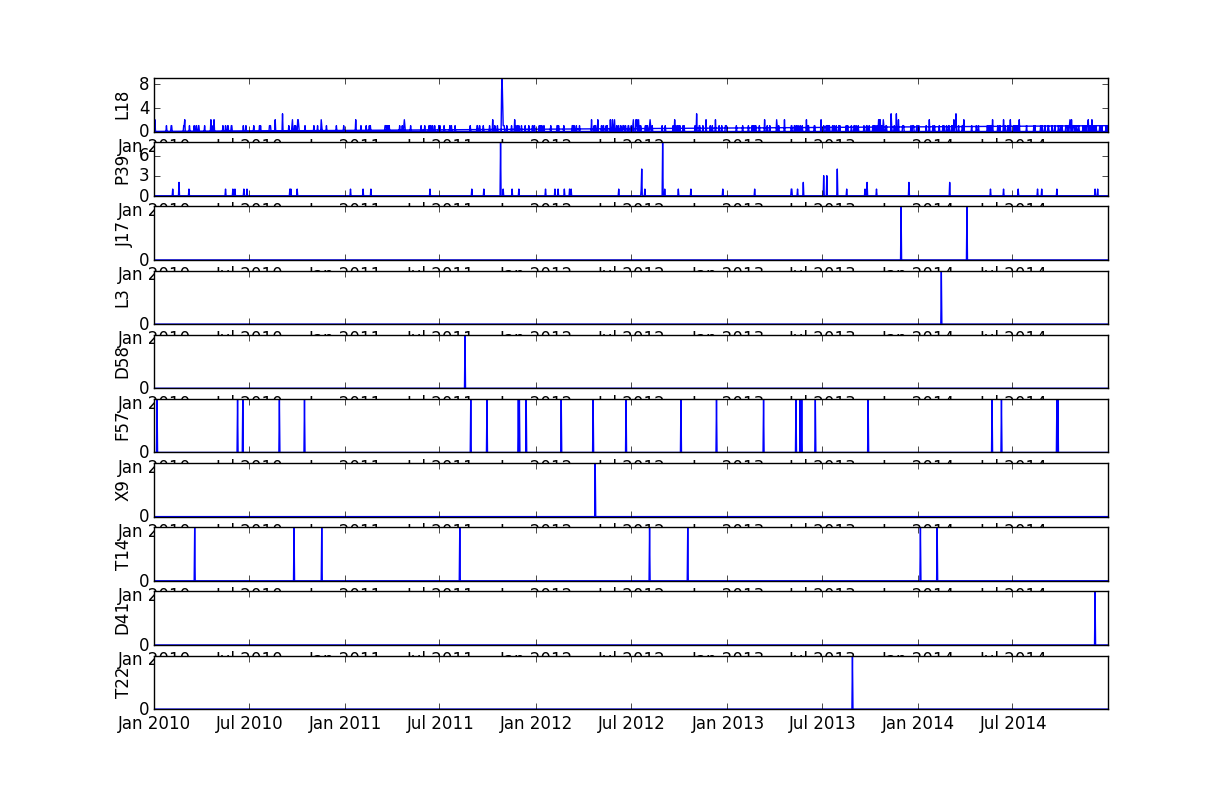
\includegraphics[width=0.99\textwidth]{../earthquakedata/output_plot/eq_ts_char.png}
\caption{Earthquake frequency in randomly sampled UTM zones in (2010-2014)}
\label{CharacterOfEarthquake}
\end{figure}



\subsection{Performance evaluation}

\subsection{Stock closing prices}

As an exploratory step, we first applied the clustering algorithms indicated in Section \ref{ExperimentalEvaluation} to the set of time series and plotted the resulting clusters side to side as shown in Figure \ref{ClusterTimeSeries}. This visualization provides insights into what stocks have common patterns and the relative ability of the different algorithms to generate relevant groups. In this case, Affinity Propagation showed the least ability to generate groups. Spectral clustering, on the other hand, achieved a spreading of the time series across multiple groups in such a way that stocks in the same group have a similar pattern.


\begin{figure}
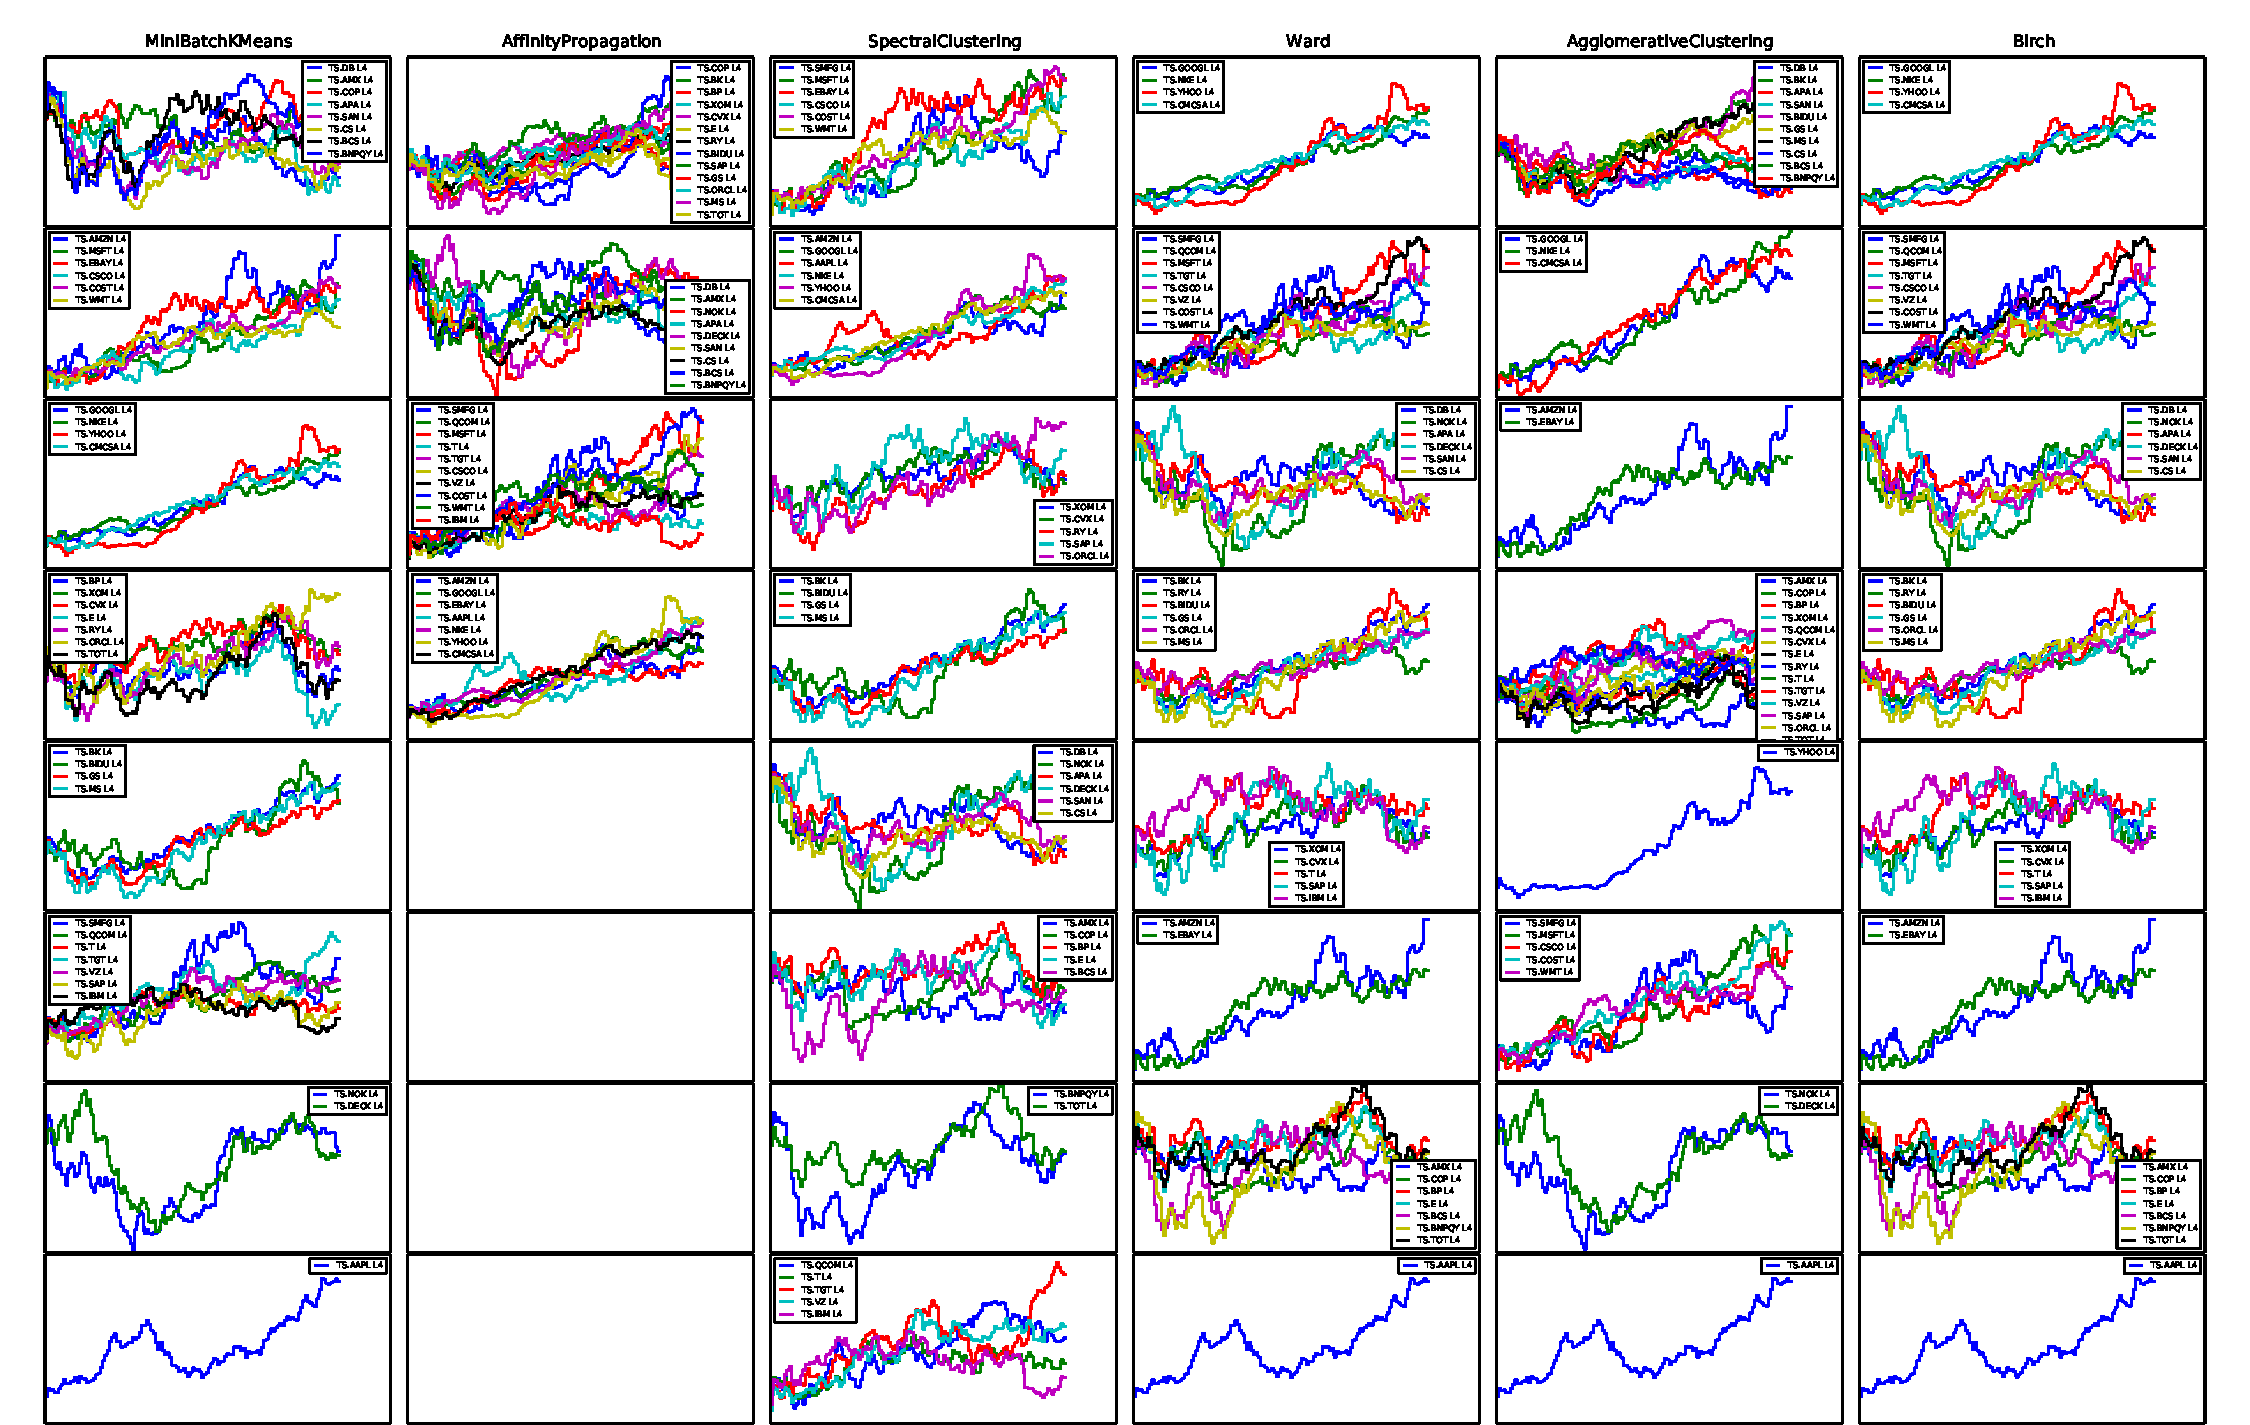
\includegraphics[width=0.99\textwidth]{../demo/CompleteGrid.pdf}
\caption{Clustering of stock closing price time series with different algorithms
using feature extraction (resolution) level four.}
\label{ClusterTimeSeries}
\end{figure}

Figure \ref{silhouette_levels} shows the impact of the clustering level and the number of clusters on the silhouette coefficient. Generally, the coefficient decreases with the number of clusters. As stocks are broken into more groups, the separation factor $b$ decreases; without a corresponding gain in cohesion $a$, the $1-a/b$ coefficient decreases. On the other hand, the silhouette coefficient is relatively insensitive to the clustering level.

Spectral Clustering, which qualitatively produced relevant clusterings (Figure \ref{ClusterTimeSeries}), has a lower coefficient than Mini-Batch K-Means, Ward and Birch. Only when the number of clusters is greater than six, its coefficient is higher than for agglomerative clustering.


\begin{figure}
\begin{center}
\subfigure[Level 2]{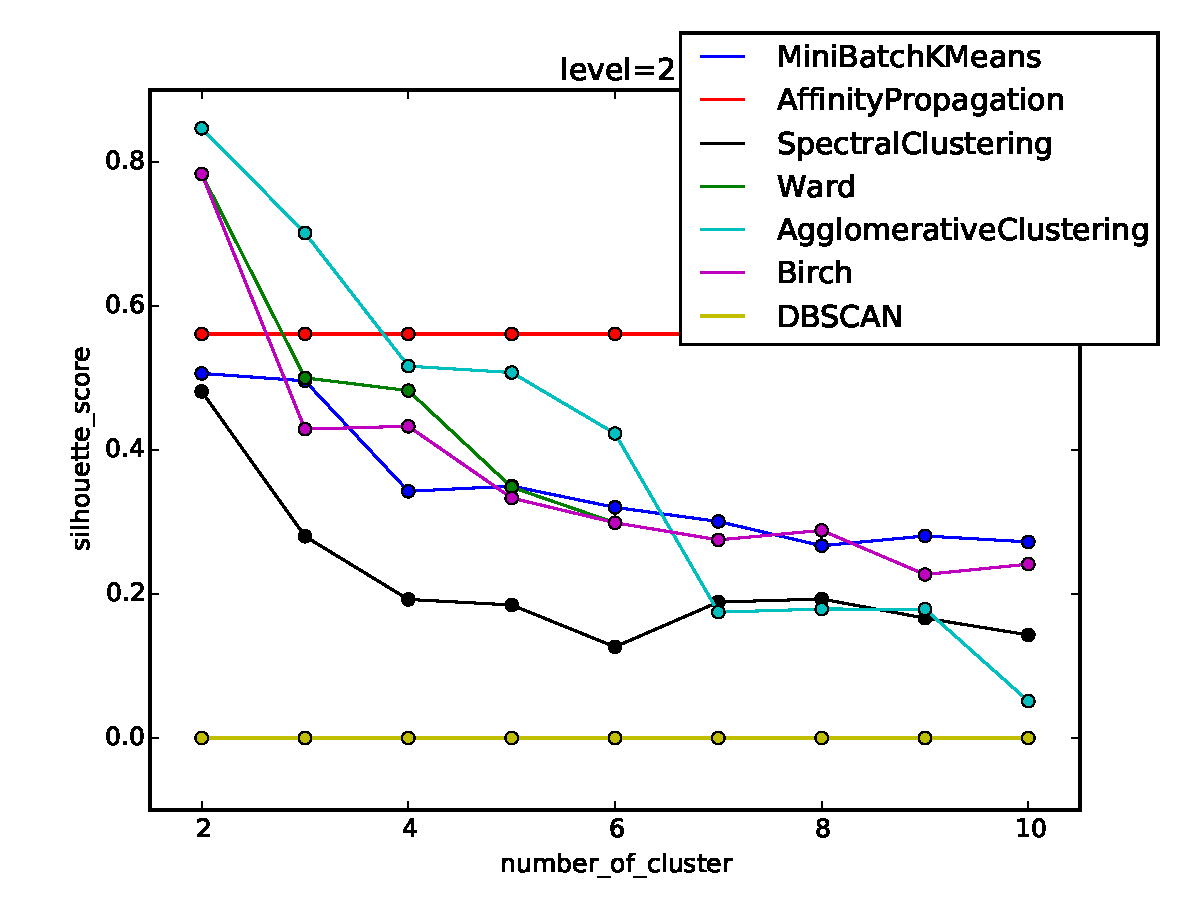
\includegraphics[width=0.49\textwidth]{../task4/silhouette_score_plot_per_number_of_cluster(level=2).pdf}}
\subfigure[Level 4]{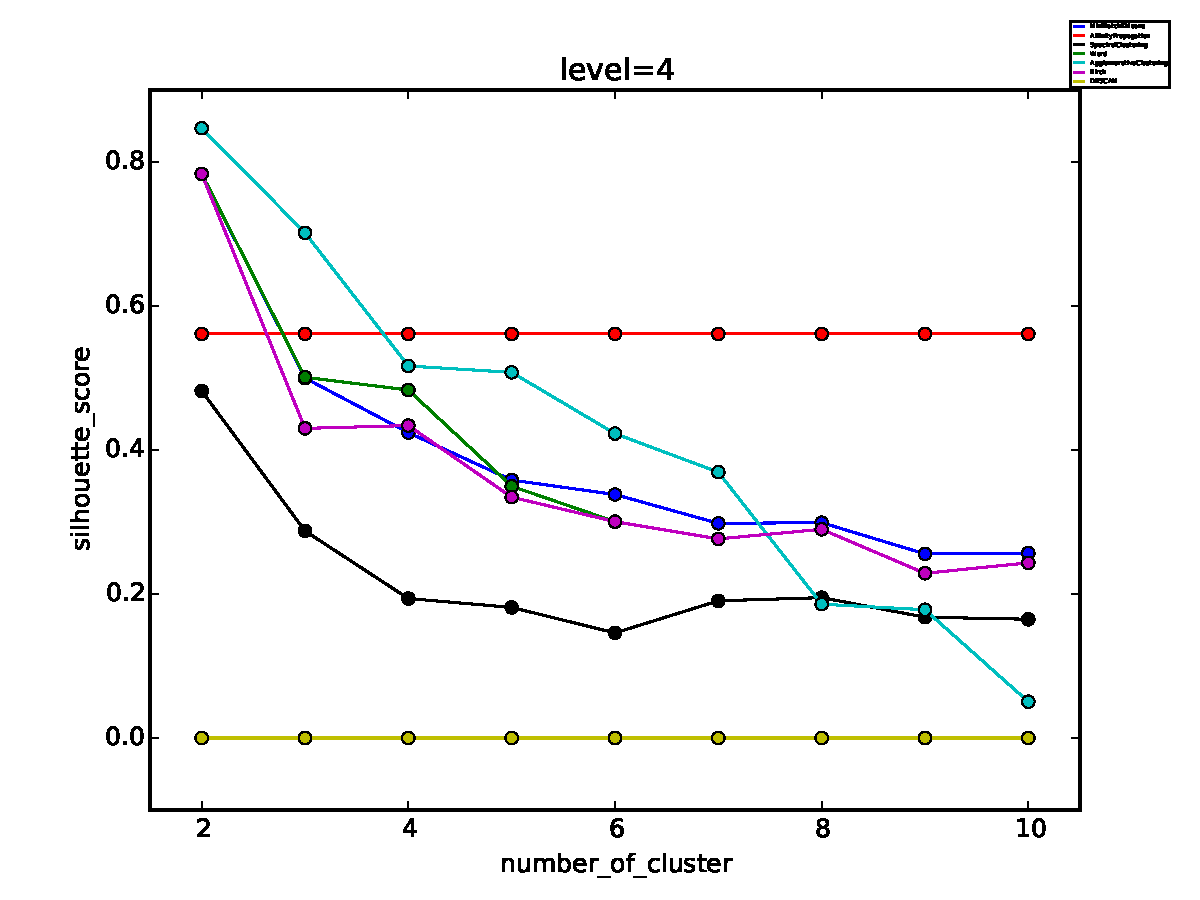
\includegraphics[width=0.49\textwidth]{../task4/silhouette_score_plot_per_number_of_cluster(level=4).pdf}}
\subfigure[Level 6]{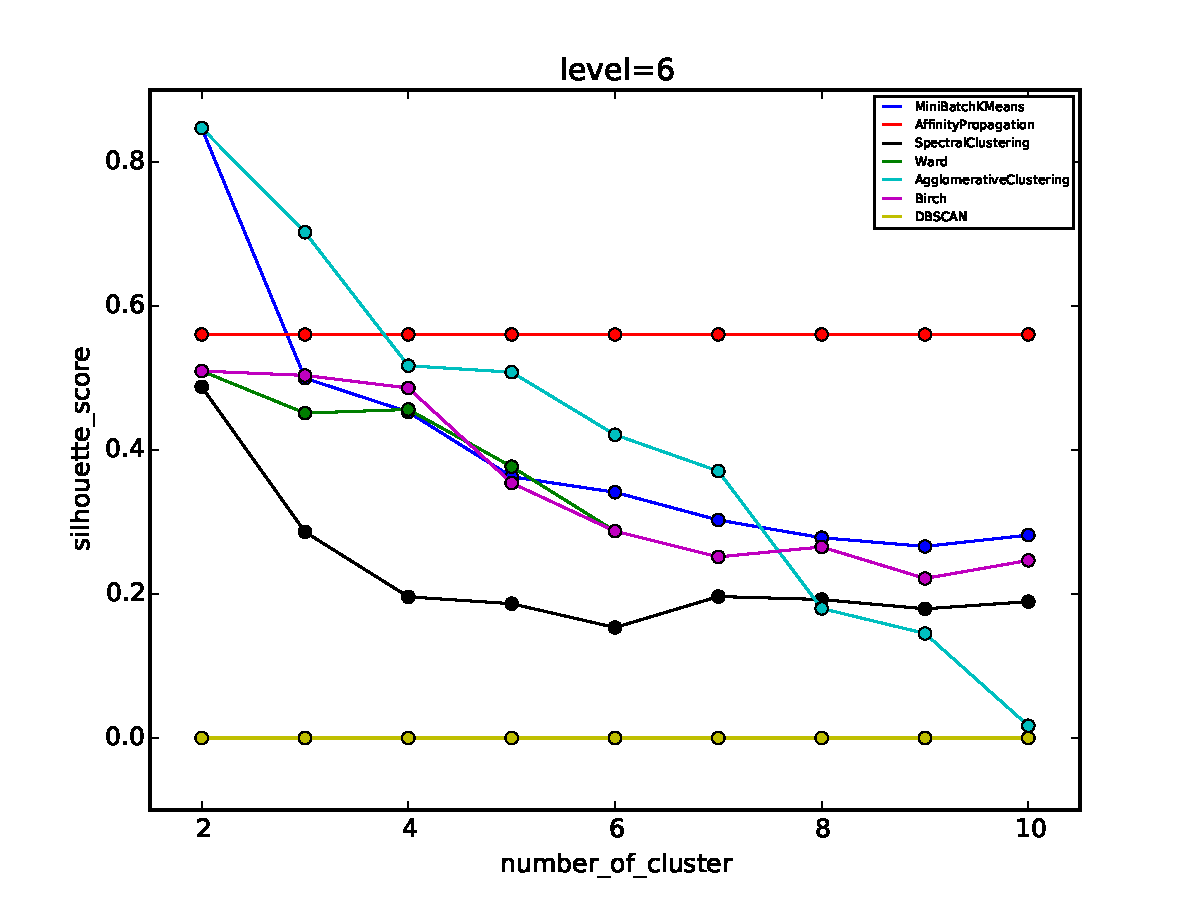
\includegraphics[width=0.49\textwidth]{../task4/silhouette_score_plot_per_number_of_cluster(level=6).pdf}}
\subfigure[Level 8]{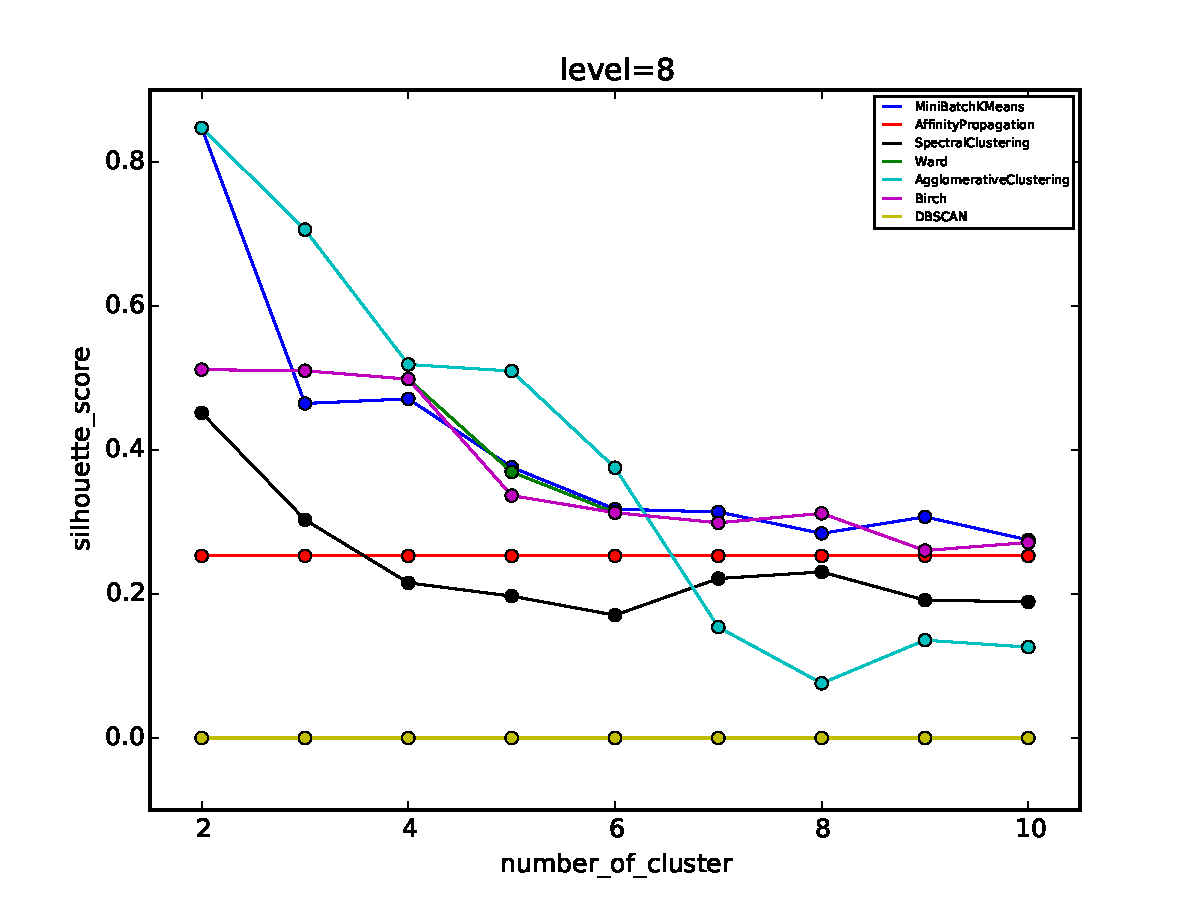
\includegraphics[width=0.49\textwidth]{../task4/silhouette_score_plot_per_number_of_cluster(level=8).pdf}}
\caption{Silhouette coefficient for various clustering levels.} \label{silhouette_levels}
\end{center}
\end{figure}

Figure \ref{silhouette_score} shows again the silhouette coefficient as a function of the clustering level and the number of clusters. As before, the coefficient decreases with the number of clusters, but is relatively insensitive to the clustering level.

\begin{figure}
\begin{center}
\subfigure[Two clusters]{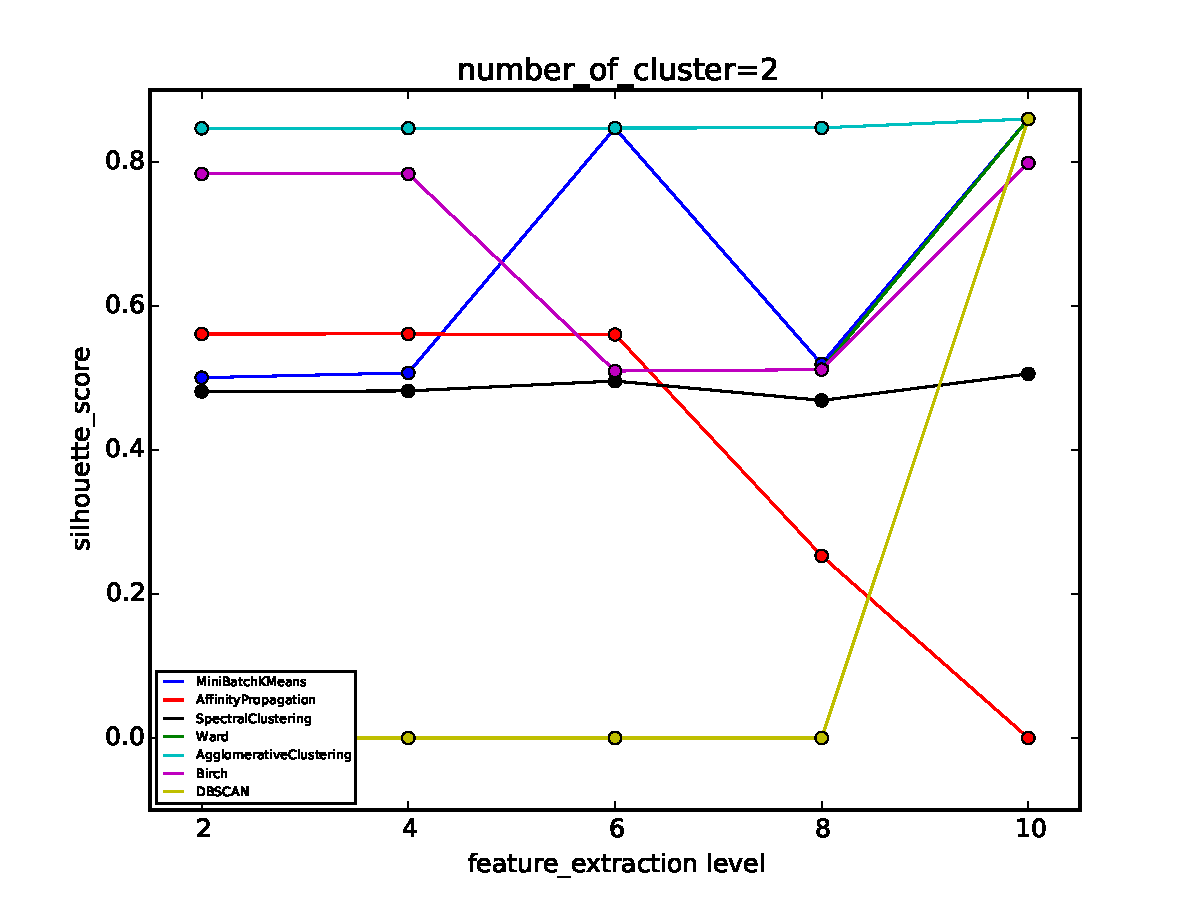
\includegraphics[width=0.49\textwidth]{../task4/silhouette_score_plot_per_level_(clusters=2).pdf}}
\subfigure[Three clusters]{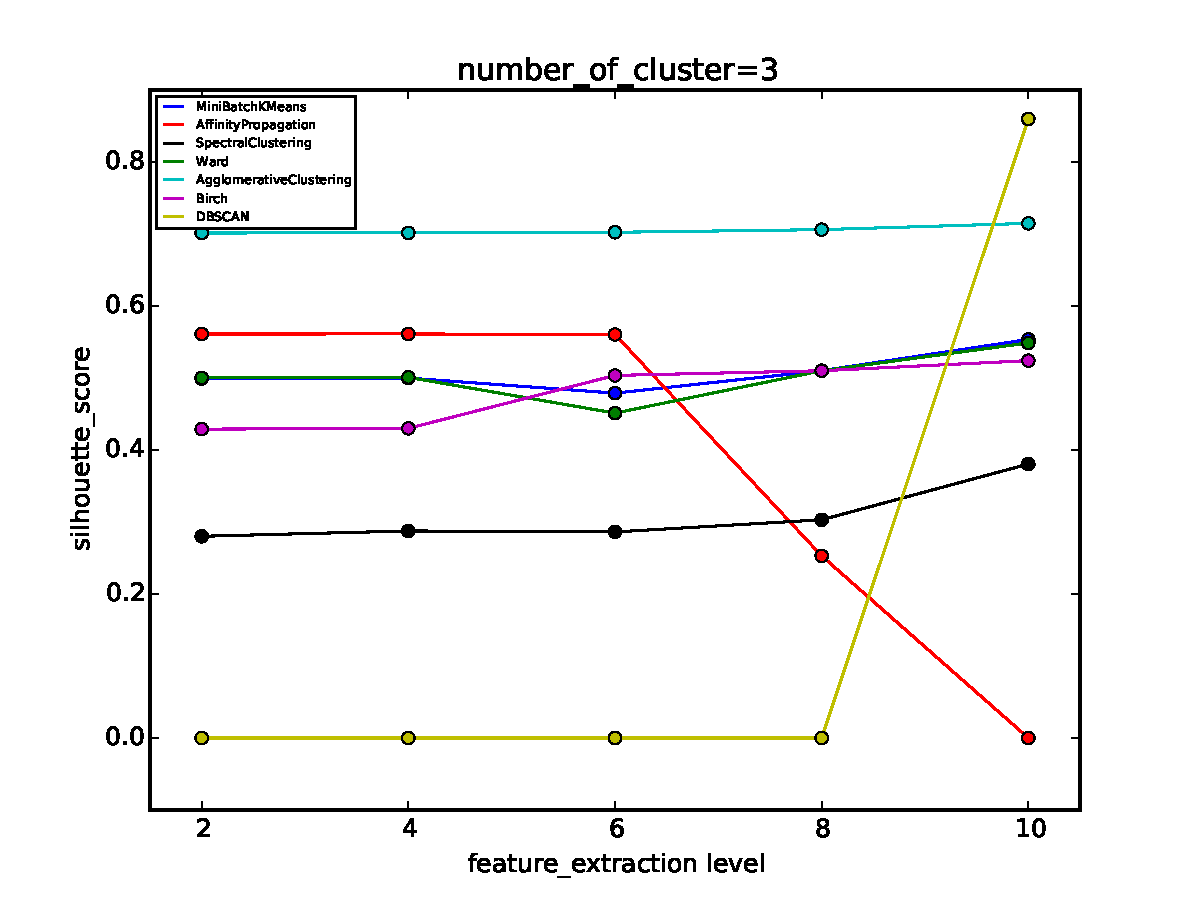
\includegraphics[width=0.49\textwidth]{../task4/silhouette_score_plot_per_level_(clusters=3).pdf}}
\subfigure[Four clusters]{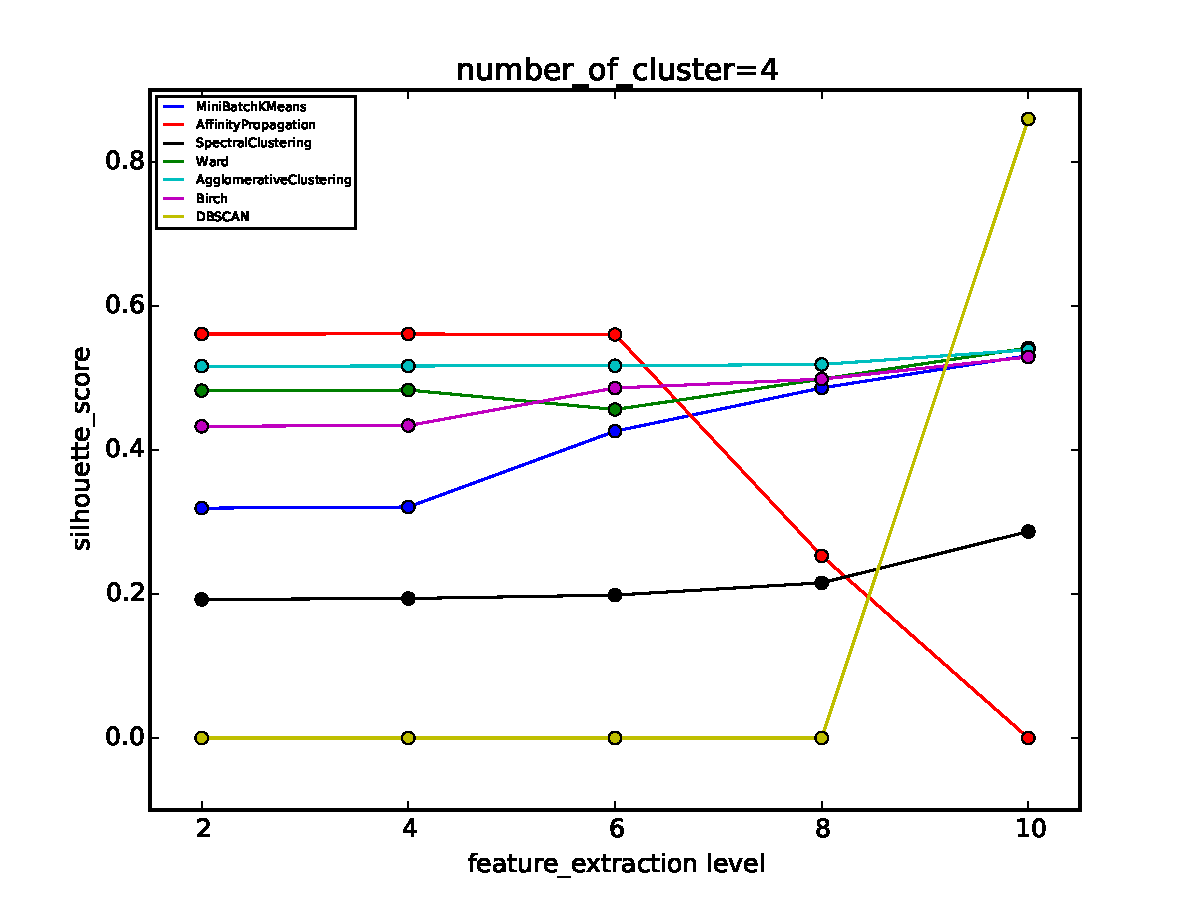
\includegraphics[width=0.49\textwidth]{../task4/silhouette_score_plot_per_level_(clusters=4).pdf}}
\subfigure[Five clusters]{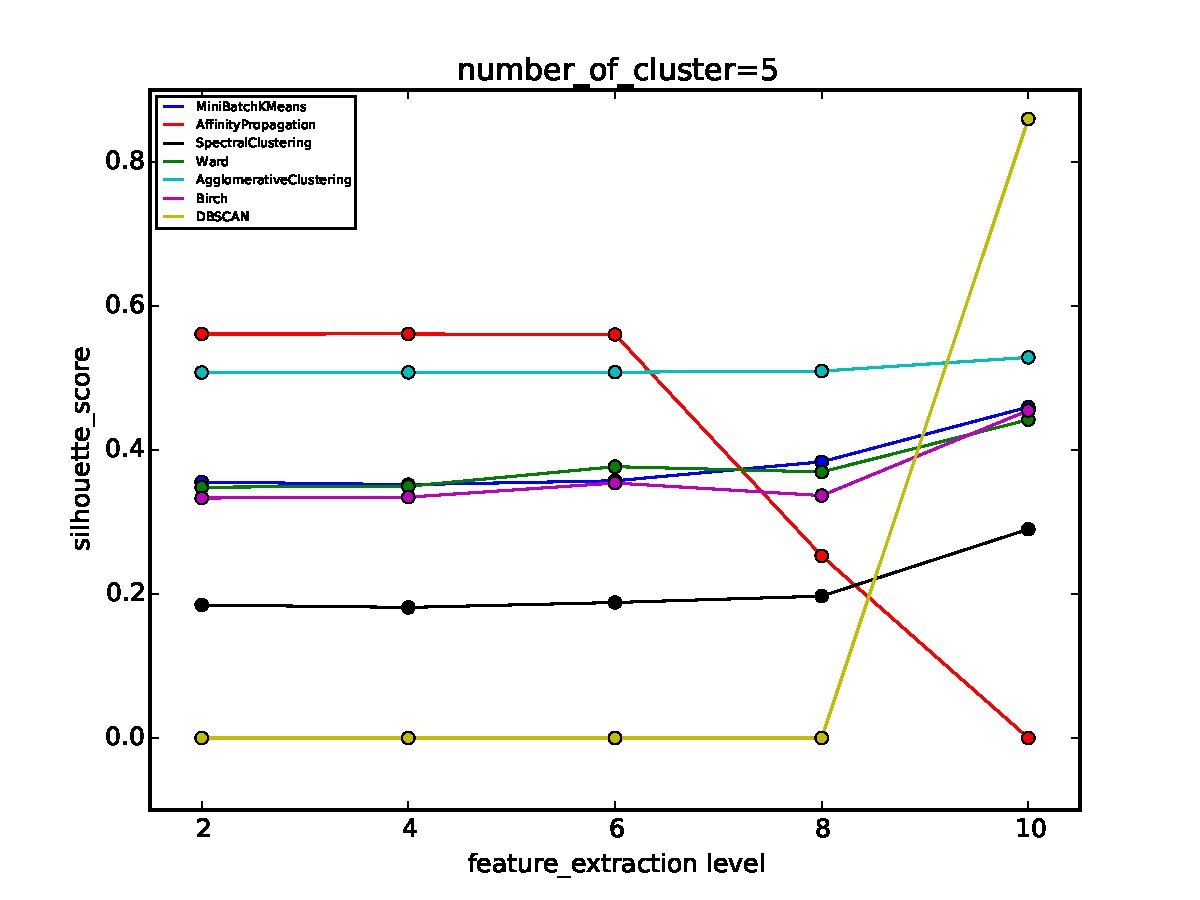
\includegraphics[width=0.49\textwidth]{../task4/silhouette_score_plot_per_level_(clusters=5).pdf}}
\subfigure[Six clusters]{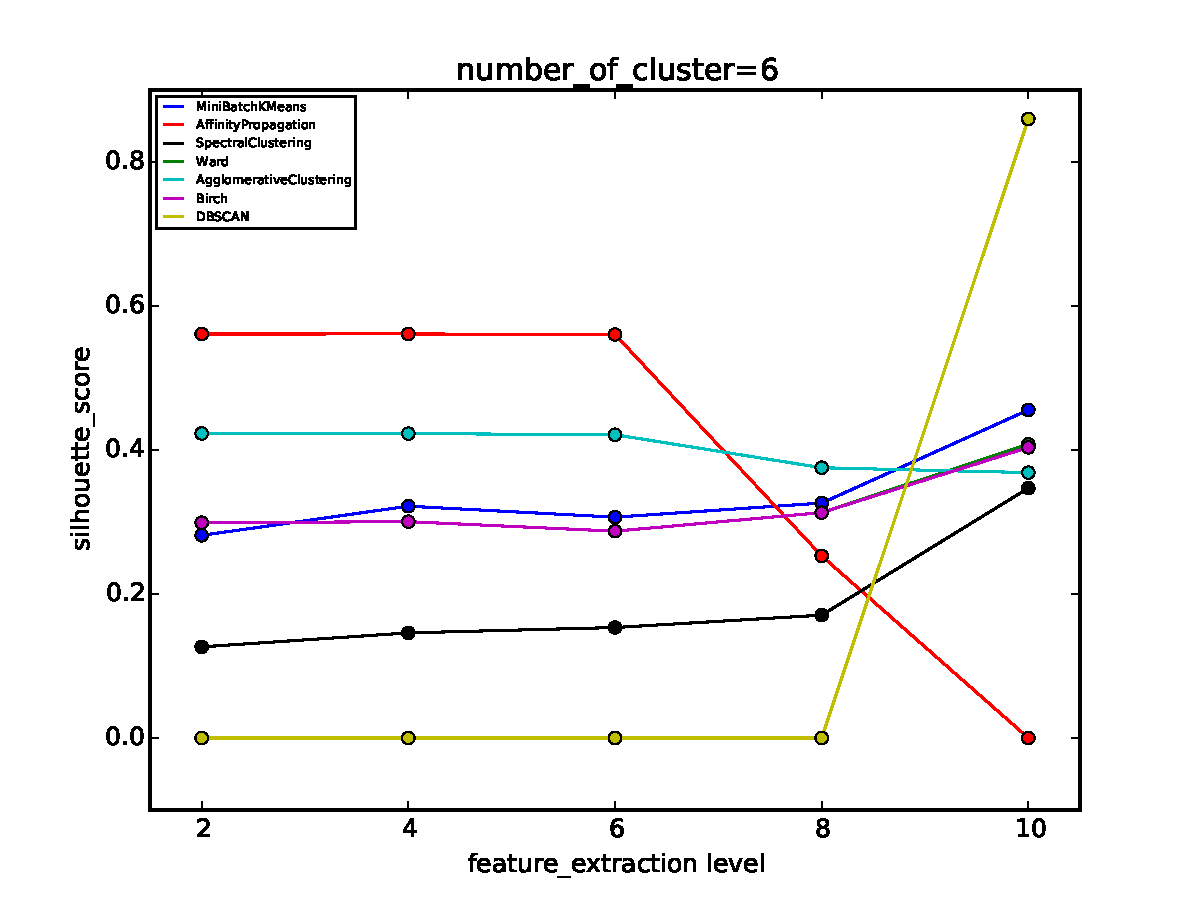
\includegraphics[width=0.49\textwidth]{../task4/silhouette_score_plot_per_level_(clusters=6).pdf}}
\subfigure[Seven clusters]{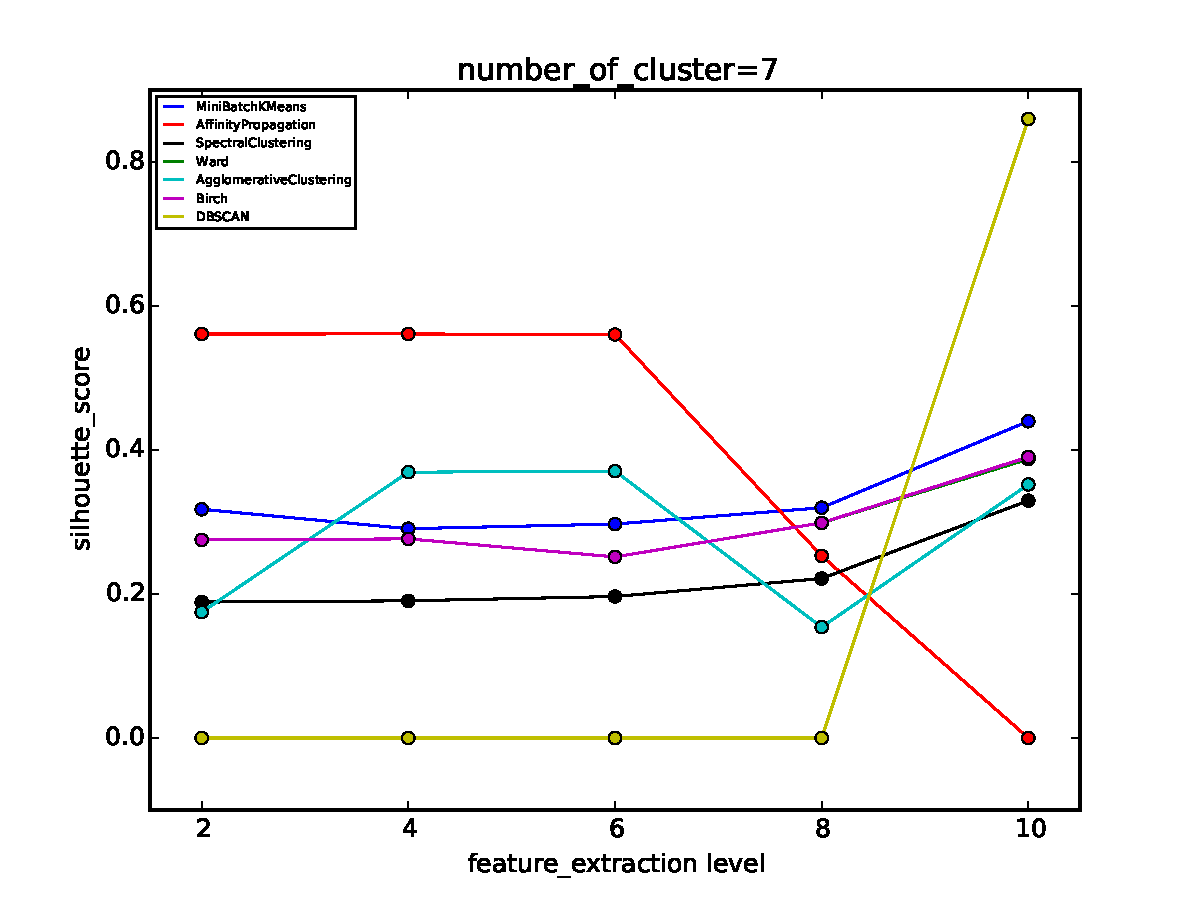
\includegraphics[width=0.49\textwidth]{../task4/silhouette_score_plot_per_level_(clusters=7).pdf}}
\subfigure[Eight clusters]{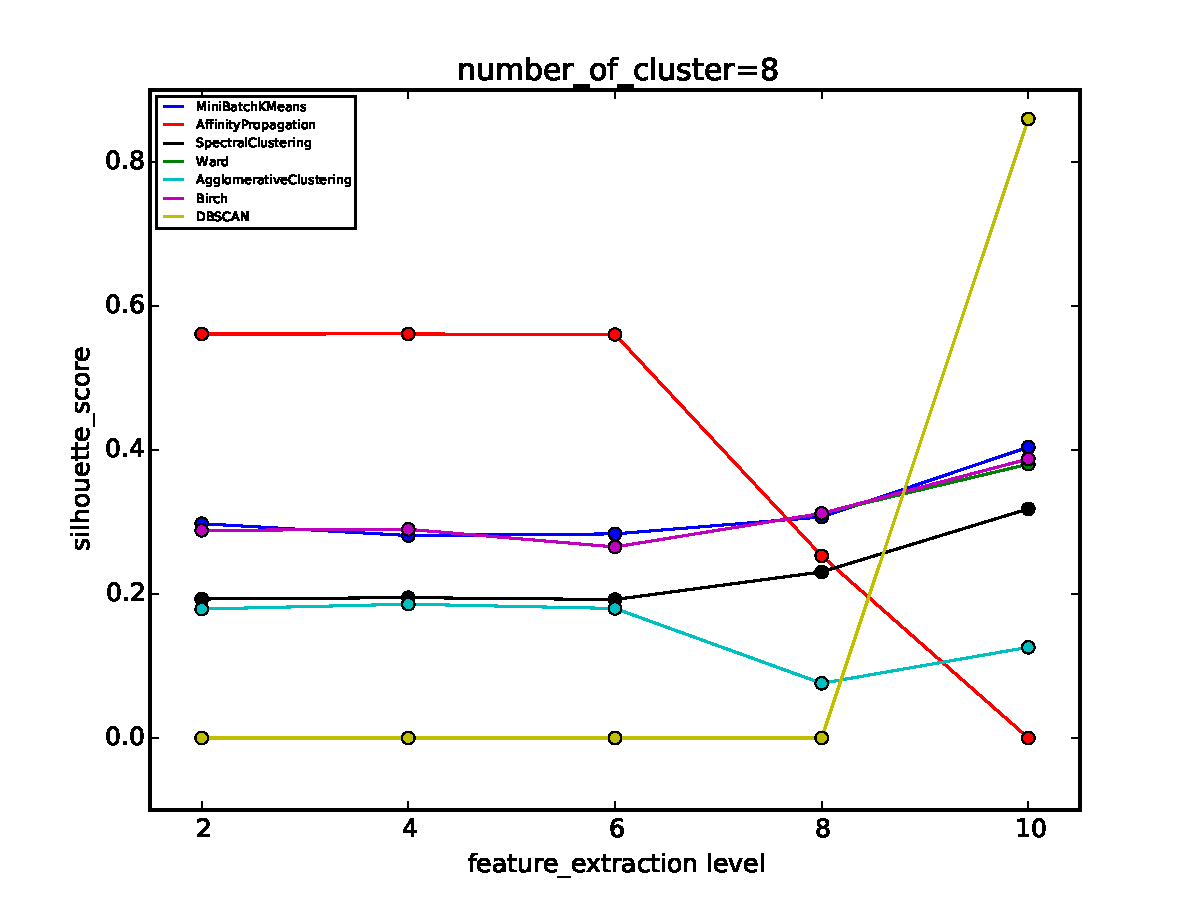
\includegraphics[width=0.49\textwidth]{../task4/silhouette_score_plot_per_level_(clusters=8).pdf}}
\subfigure[Nine clusters]{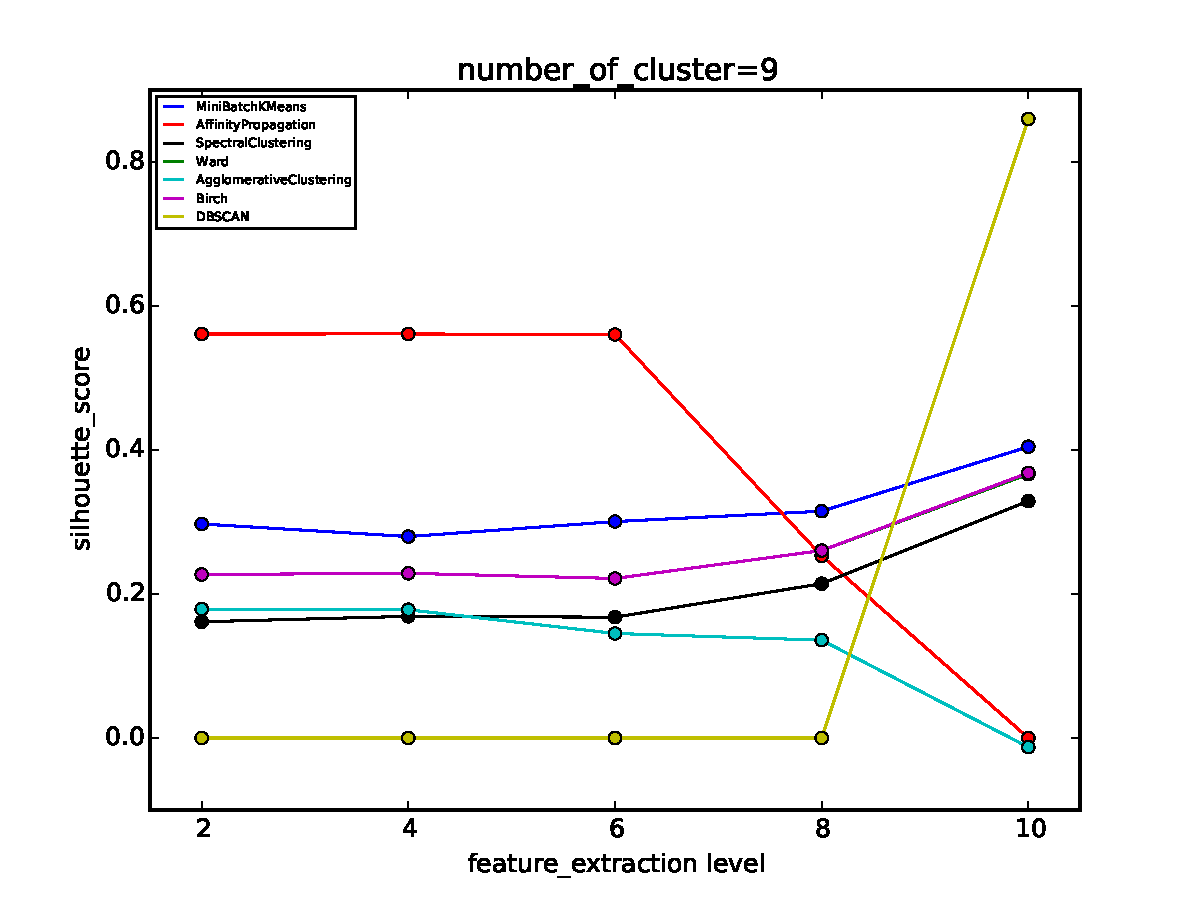
\includegraphics[width=0.49\textwidth]{../task4/silhouette_score_plot_per_level_(clusters=9).pdf}}
\caption{Silhouette coefficient for various clustering levels.} \label{silhouette_score}
\end{center}
\end{figure}



\subsection{Historic exchange rates}
Lorem ipsum dolor sit amet, consectetur adipiscing elit, sed do eiusmod tempor incididunt ut labore et dolore magna aliqua. Ut enim ad minim veniam, quis nostrud exercitation ullamco laboris nisi ut aliquip ex ea commodo consequat. Duis aute irure dolor in reprehenderit in voluptate velit esse cillum dolore eu fugiat nulla pariatur. Excepteur sint occaecat cupidatat non proident, sunt in culpa qui officia deserunt mollit anim id est laborum.


\subsection{Historic earthquake data}
On earthquake frequency dataset, we applied a few clustering algorithm to explore relation between clustering and geological distance. Geologically surface of our earth are consisted of some plates, earthquakes are caused by movements of those plates. Therefore, UTM zones might be classified by whether they are on the same boundary of plates more than by they distance.
Figure \ref{EarthquakeWorldMap} shows the UTM-zone in each cluster. Points in the same color indicates, the UTM-zones in the same cluster. Figure \ref{PlateWorldMap} shows tectonic plates of our earth \cite{WTP15}. As shown in Figure 2010-2014 Kmeans of \ref{EarthquakeWorldMap},
we can find some implicit trends that UTM points, on the same boundary in Figure \ref{PlateWorldMap}, are classified in the same cluster.

\begin{figure}
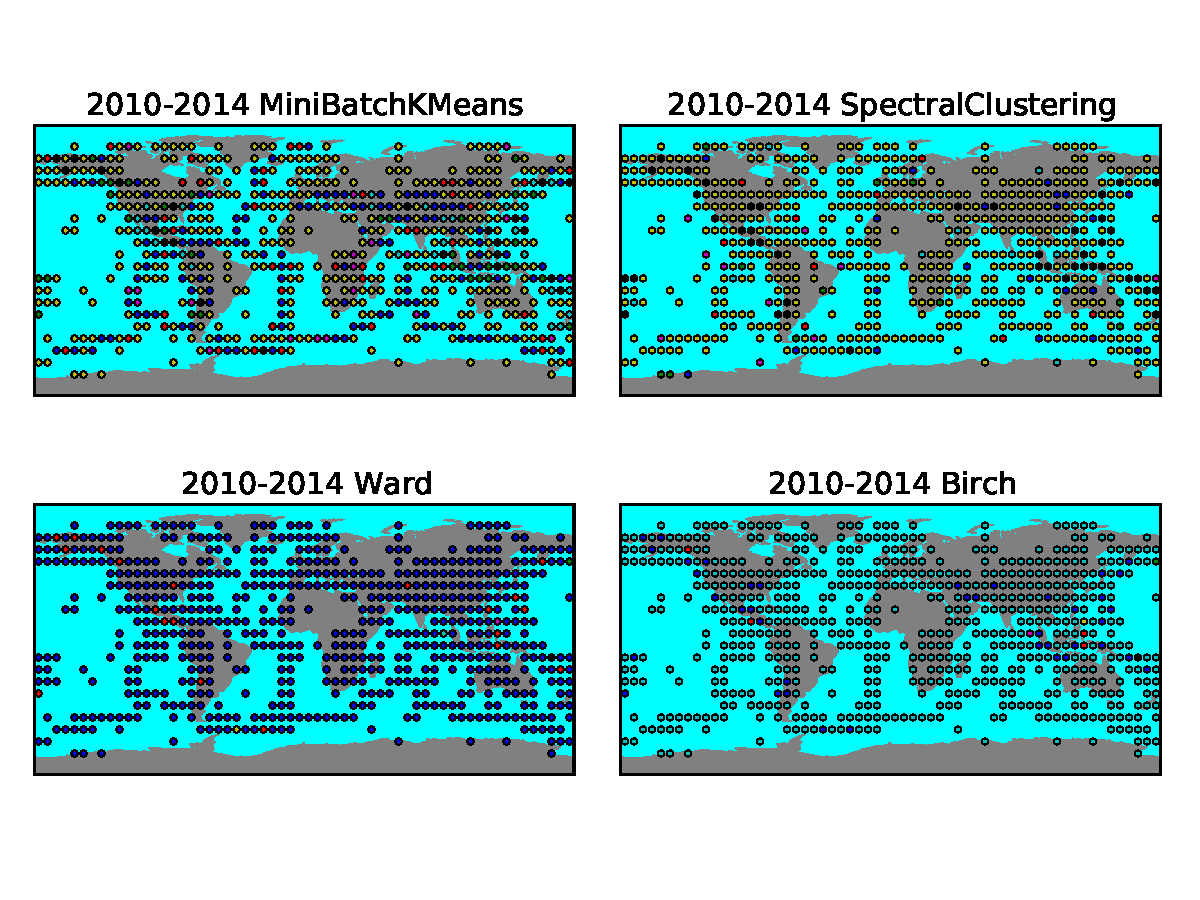
\includegraphics[width=0.99\textwidth]{../earthquakedata/output_map_plot/grid(year=2010-2014,level=6,number_of_cluster=7).pdf}
\caption{Clustering of earthquake frequency per day with different algorithms
using feature extraction (resolution) level six, number of clusters seven.}
\label{EarthquakeWorldMap}
\end{figure}

\begin{figure}
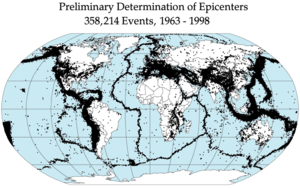
\includegraphics[width=0.99\textwidth]{../earthquakedata/output_map_plot/Tectonic_plates_boundaries.png}
\caption{Plate tectonic map of our earth.}
\label{PlateWorldMap}
\end{figure}

Clustering map contains information of not only tectonic plates geology, but also cluster changes over years. 
Figure \ref{Cluster2010vs.2013} shows that clusters in 2010 are migrated in a cluster in 2013. We can assume that earthquake are more related to each other over years by some external causes, such as increasing number of mining on the earth.

\begin{figure}[H]
\centering
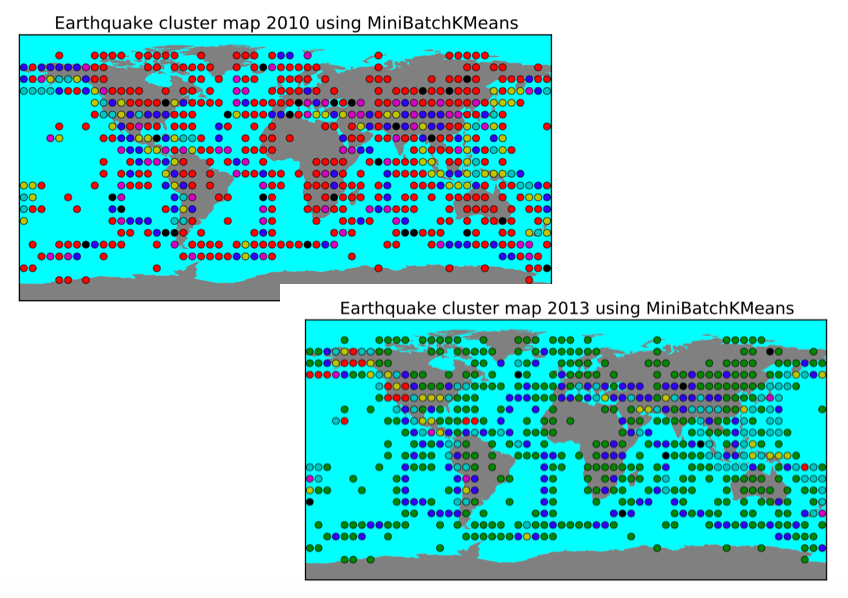
\includegraphics[width=0.99\textwidth]{../earthquakedata/output_map_plot/MiniBatchKMeans(year=2010,2013,level=6,number_of_cluster=7).png}
\caption{Clustering of earthquake frequency per day in 2010 vs. 2014 with K-mean
using feature extraction (resolution) level six, number of clusters seven.}
\label{Cluster2010vs.2013}
\end{figure}

Next, we find out what algorithms and parameter setting are fit to earthquake dataset. Figure \ref{silhouette_levels_eq} shows the impact of the clustering level and the number of clusters on the silhouette coefficient. Clustering algorithms are not affected by number of clusters as much as stock price data is affected, except for k-mean clustering. K-means shows drastic changes when the number of cluster is small, since there are geologically a few plates.

\begin{figure}[H]
\centering
\subfigure[Level 2]{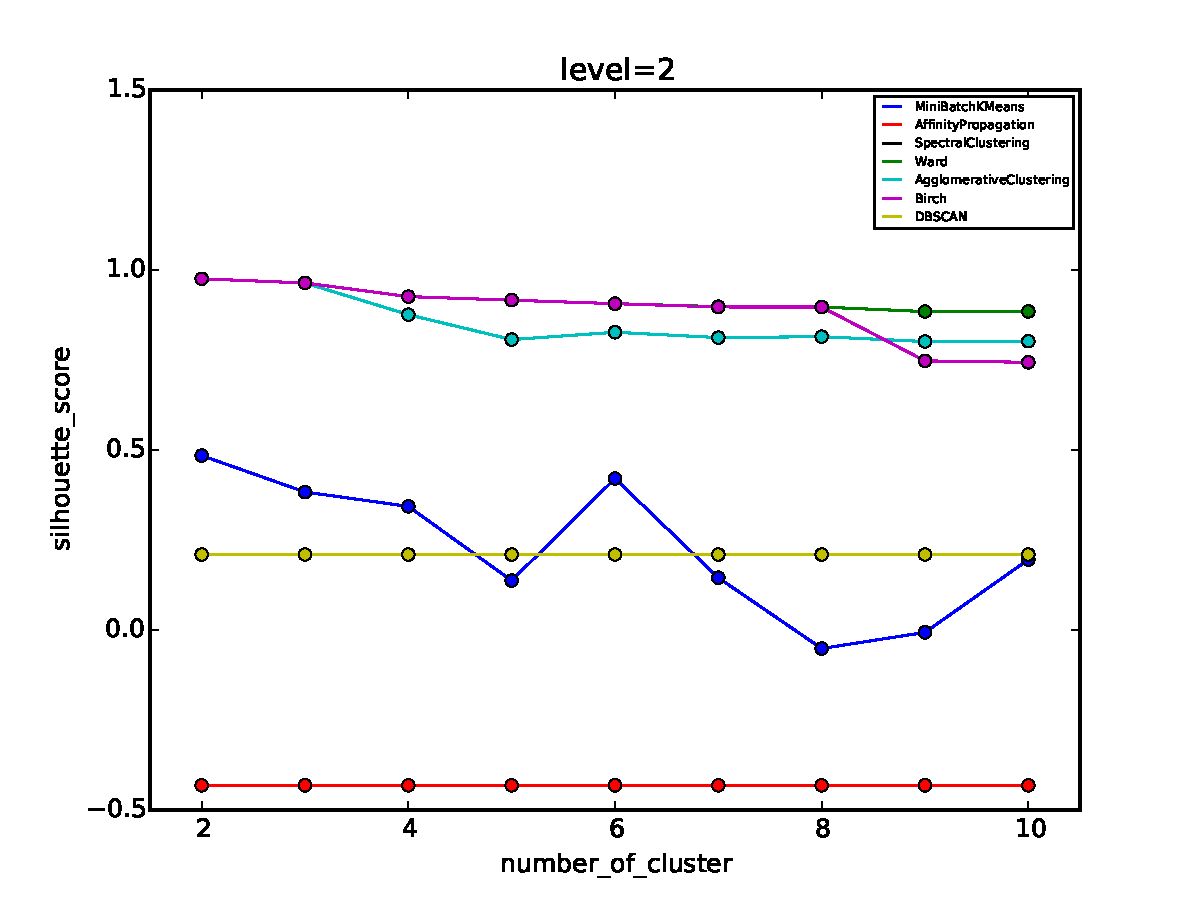
\includegraphics[width=0.49\textwidth]{../earthquakedata/output_plot/silhouette_score_plot_per_number_of_cluster(level=2).pdf}}
\subfigure[Level 4]{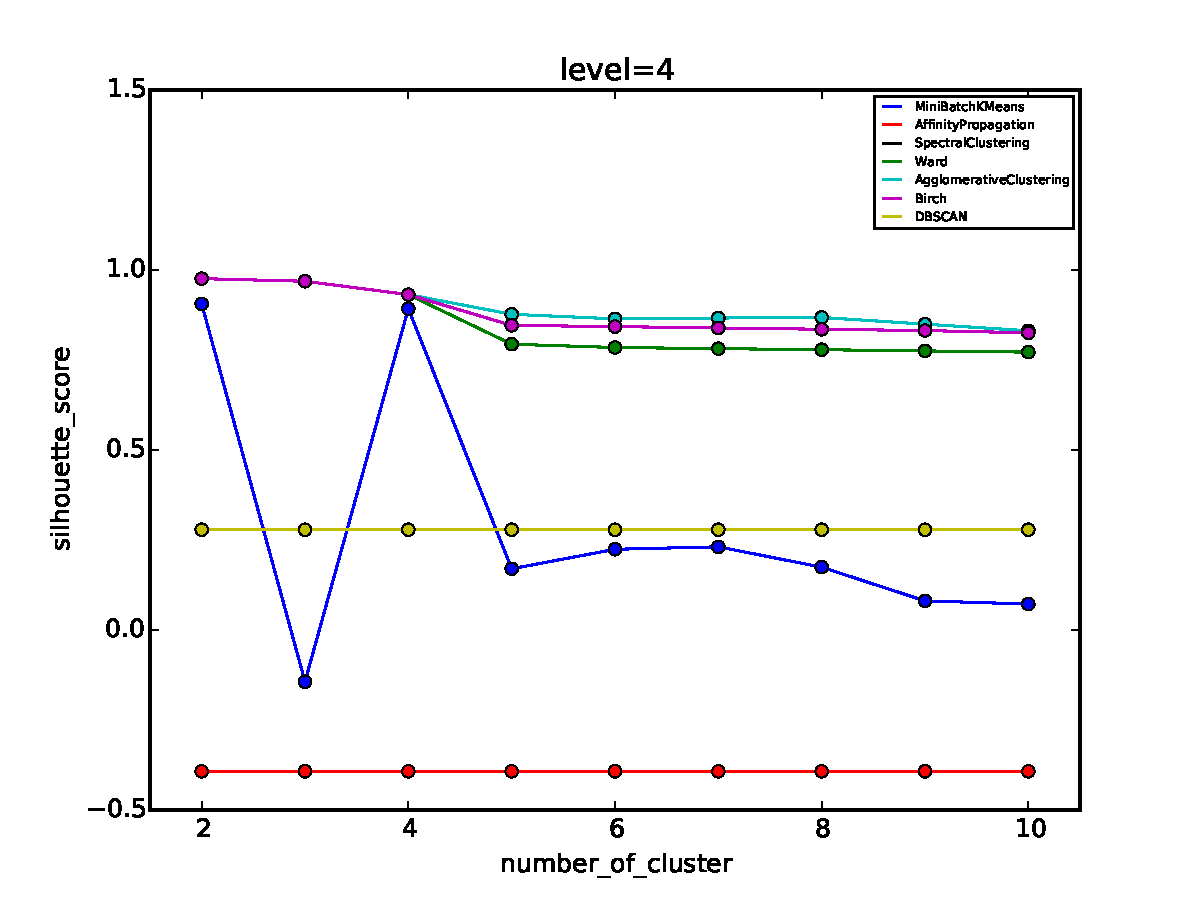
\includegraphics[width=0.49\textwidth]{../earthquakedata/output_plot/silhouette_score_plot_per_number_of_cluster(level=4).pdf}}
\subfigure[Level 6]{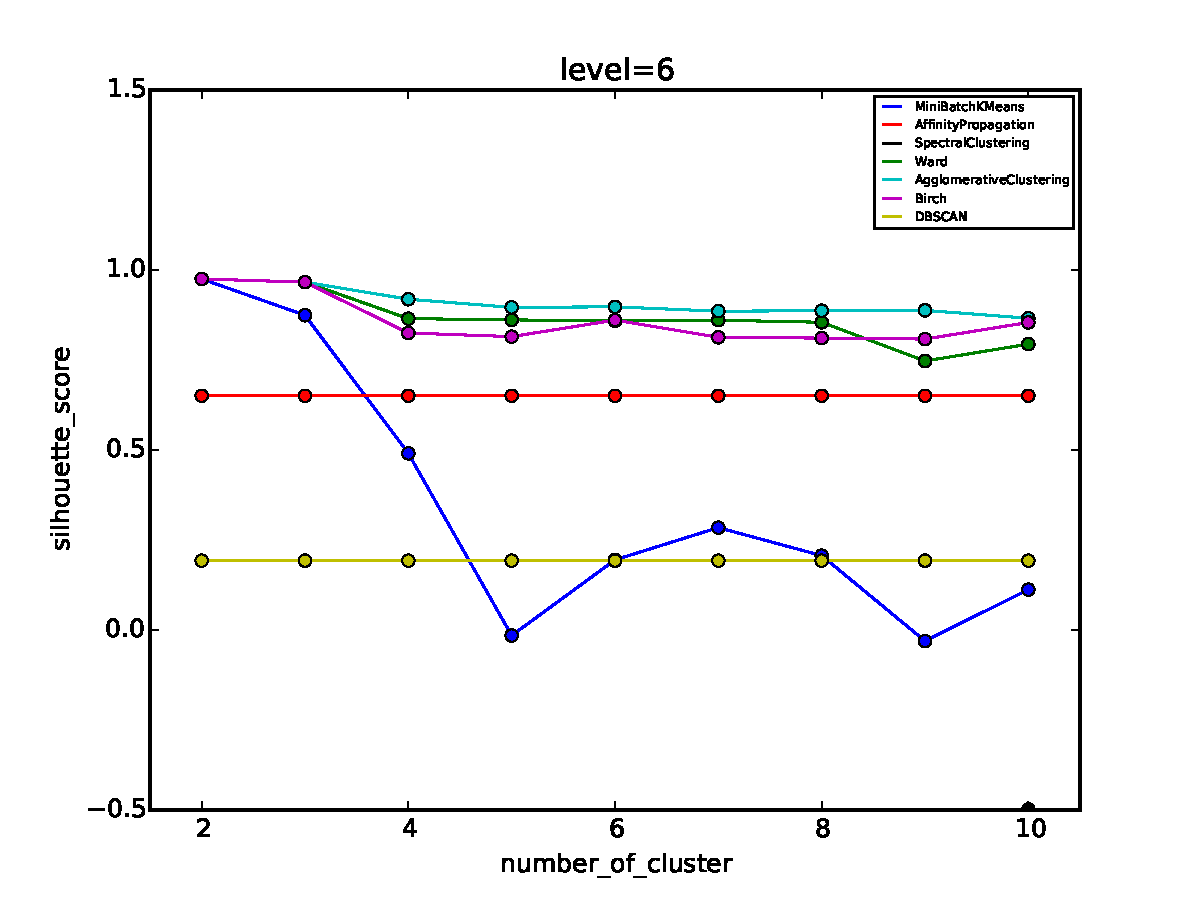
\includegraphics[width=0.49\textwidth]{../earthquakedata/output_plot/silhouette_score_plot_per_number_of_cluster(level=6).pdf}}
\subfigure[Level 8]{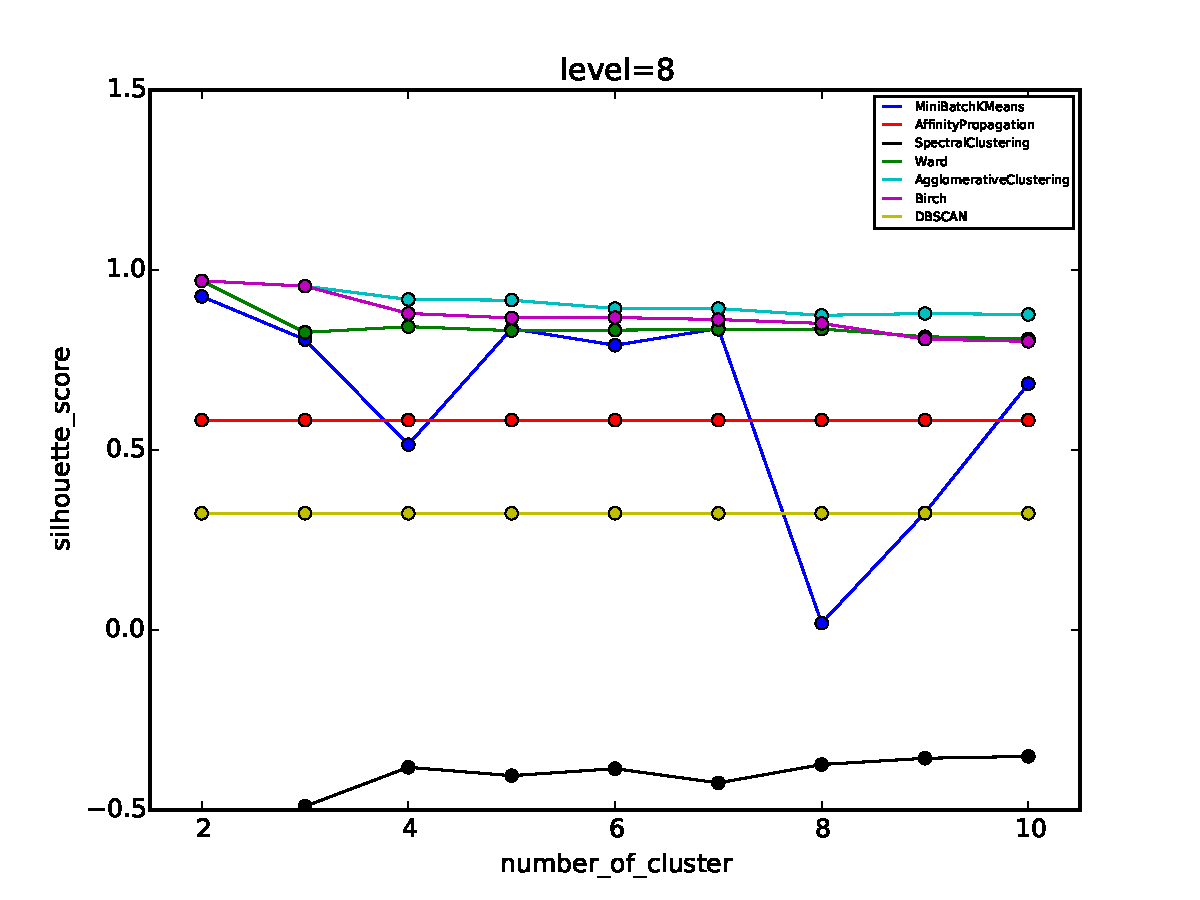
\includegraphics[width=0.49\textwidth]{../earthquakedata/output_plot/silhouette_score_plot_per_number_of_cluster(level=8).pdf}}
\caption{Silhouette coefficient for various clustering levels on earthquake frequency dataset.} \label{silhouette_levels_eq}
\end{figure}

Figure \ref{silhouette_score_eq} shows again the silhouette coefficient as a function of the clustering level and the number of clusters. Unlike the Figure \ref{silhouette_score} of stock price, earthquake data set is fit to clustering algorithms with high feature extraction level (low resolution), since earthquake frequency dataset are zero at most case, and there are earthquake in each UTM-zone for only a few days a month or a year. The higher level of feature extraction is, the better we can describe earthquake frequency data.

\begin{figure}[H]
\centering
\subfigure[Two clusters]{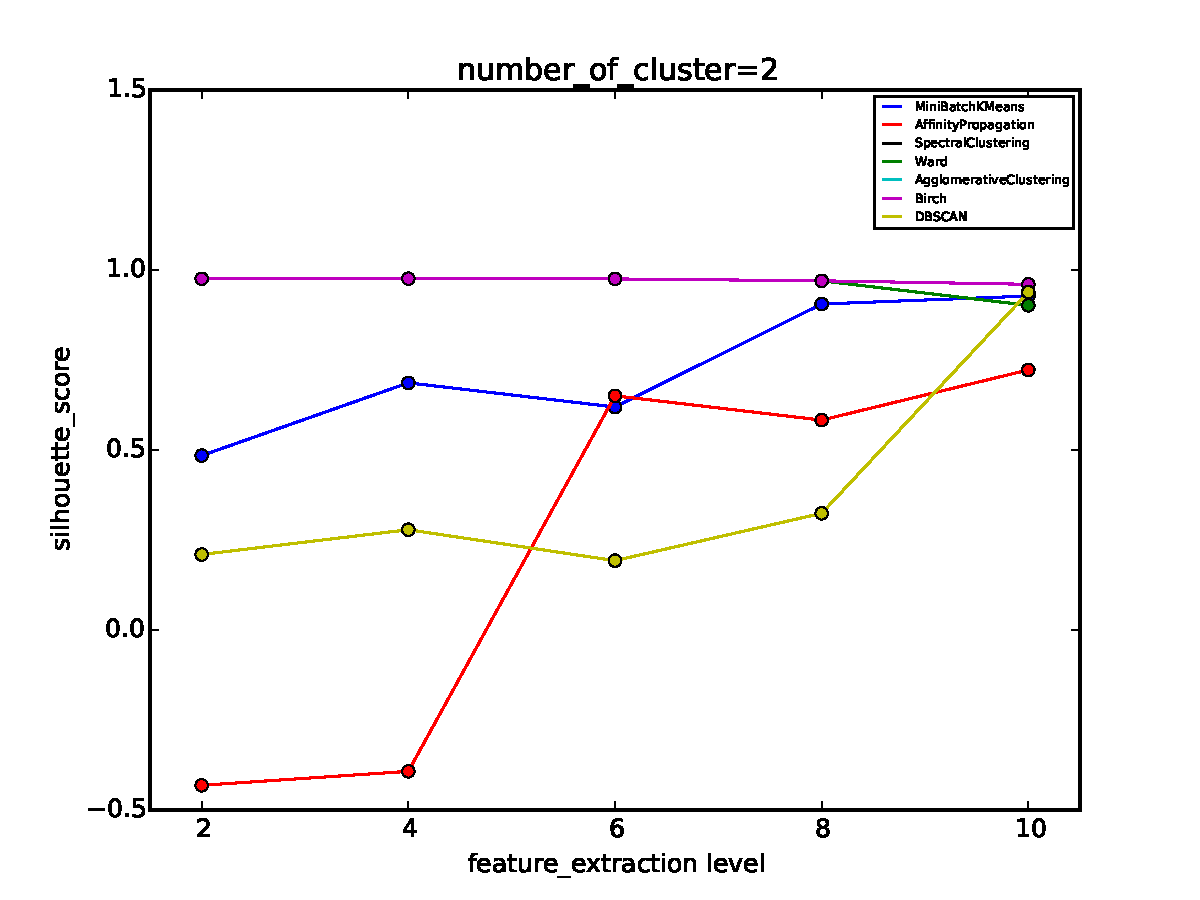
\includegraphics[width=0.49\textwidth]{../earthquakedata/output_plot/silhouette_score_plot_per_level_(clusters=2).pdf}}
\subfigure[Three clusters]{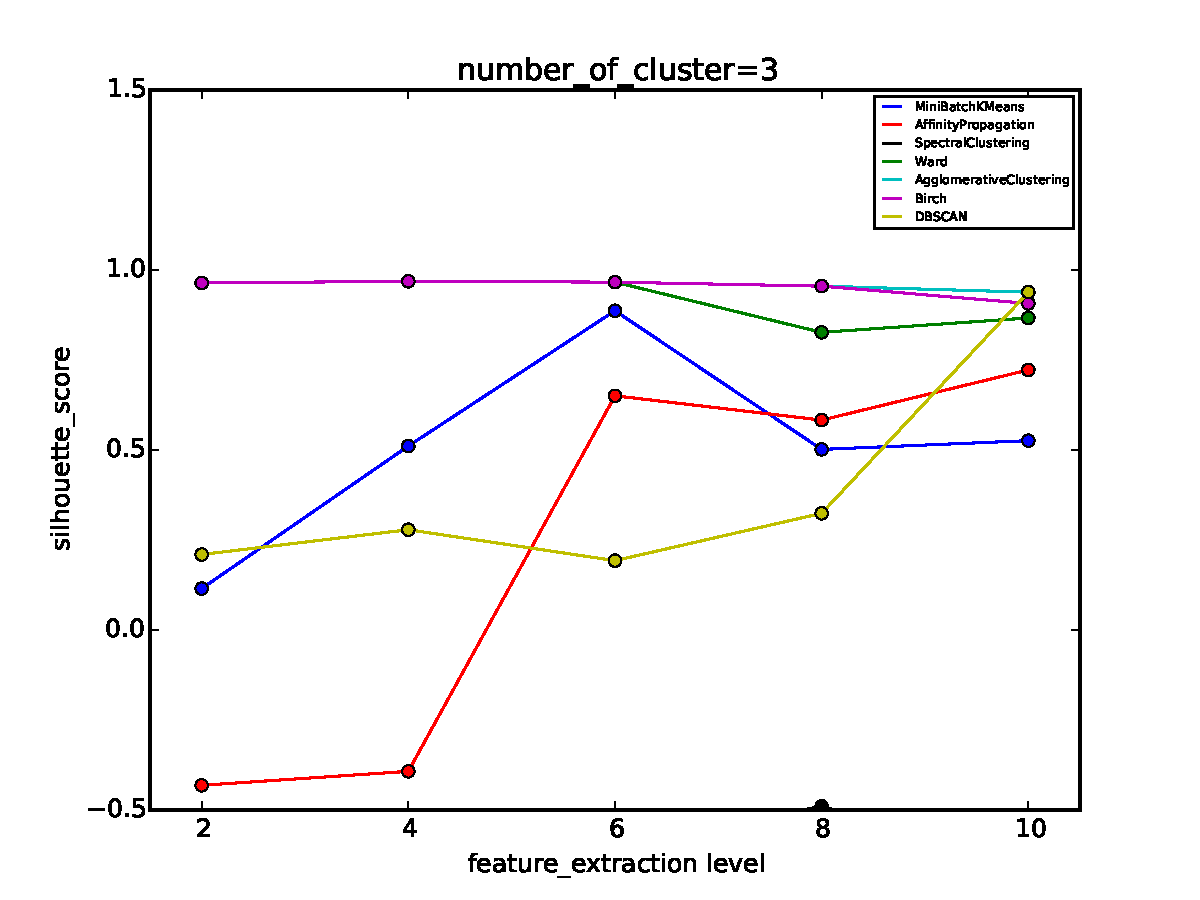
\includegraphics[width=0.49\textwidth]{../earthquakedata/output_plot/silhouette_score_plot_per_level_(clusters=3).pdf}}
\subfigure[Four clusters]{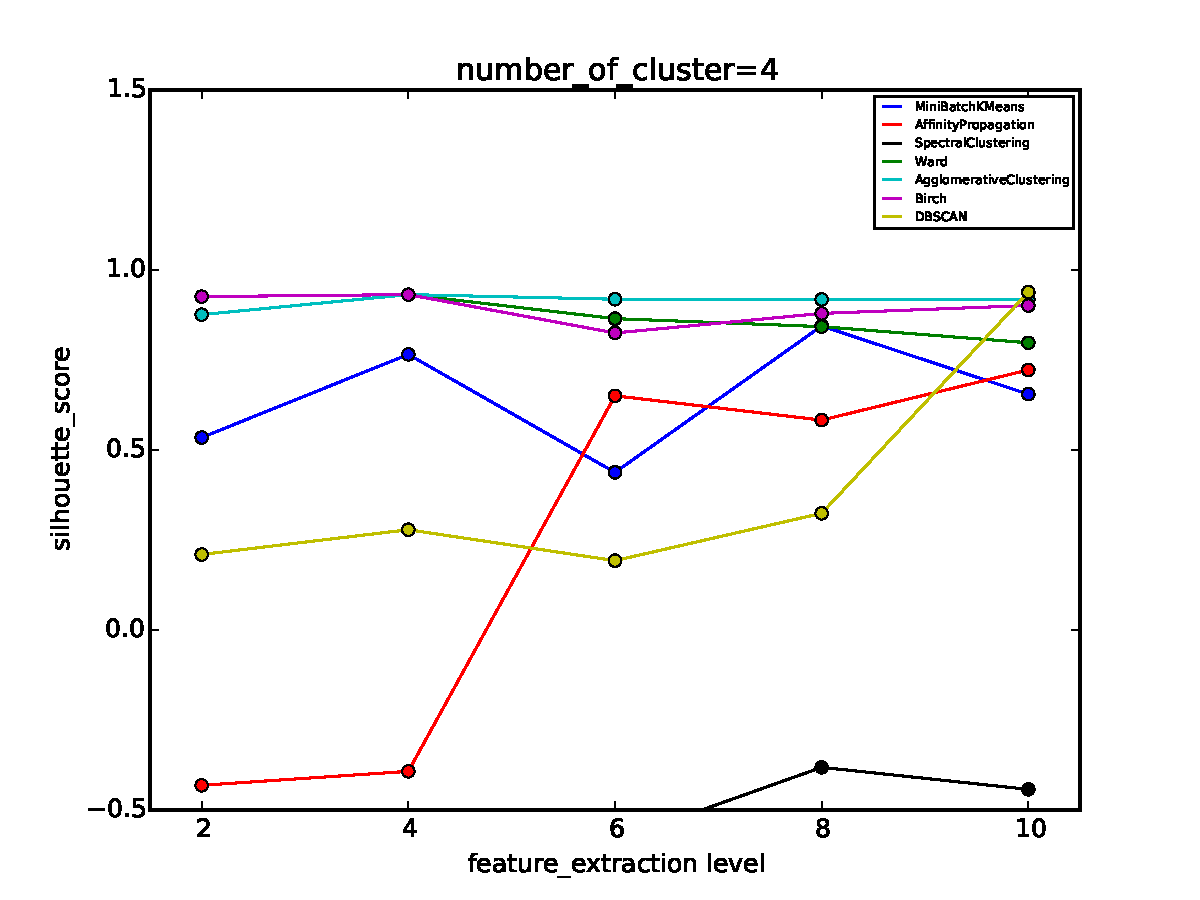
\includegraphics[width=0.49\textwidth]{../earthquakedata/output_plot/silhouette_score_plot_per_level_(clusters=4).pdf}}
\subfigure[Five clusters]{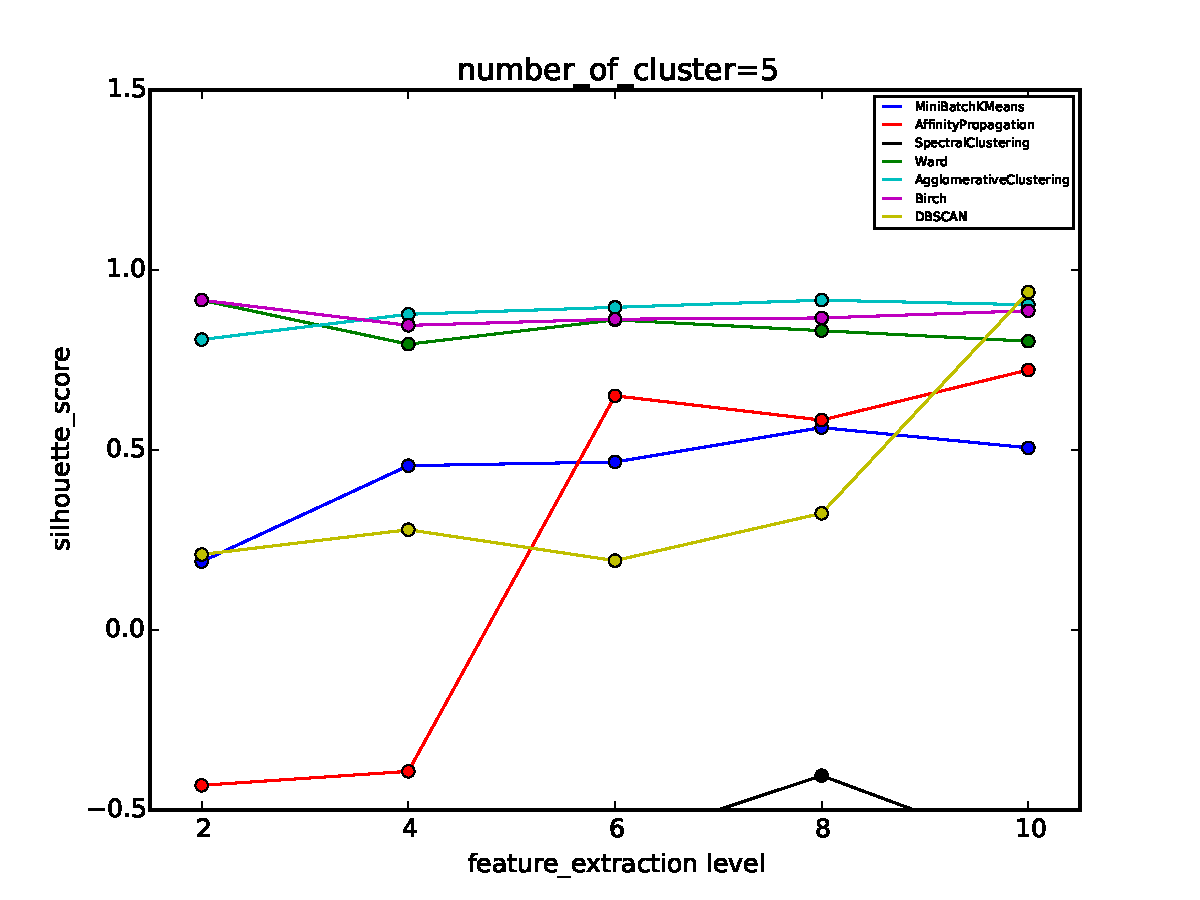
\includegraphics[width=0.49\textwidth]{../earthquakedata/output_plot/silhouette_score_plot_per_level_(clusters=5).pdf}}
\subfigure[Six clusters]{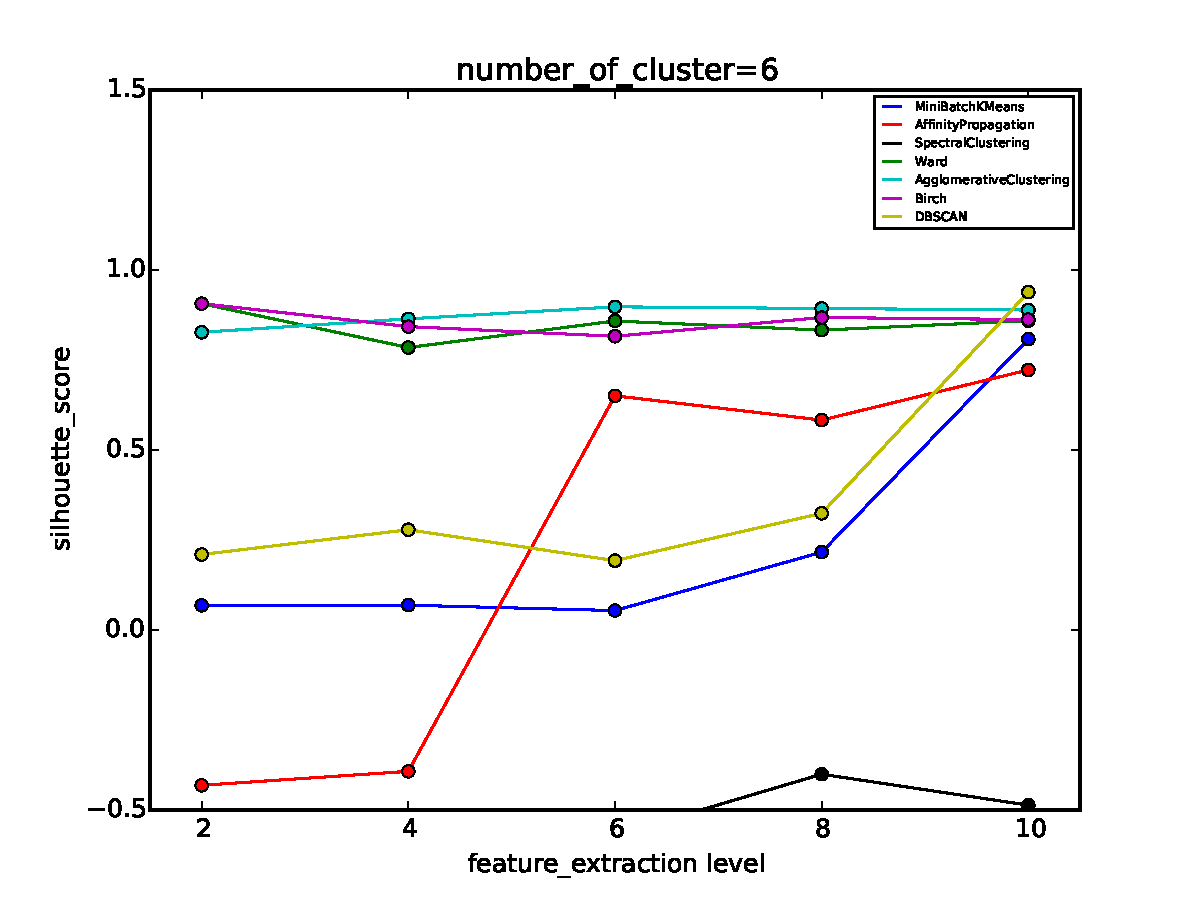
\includegraphics[width=0.49\textwidth]{../earthquakedata/output_plot/silhouette_score_plot_per_level_(clusters=6).pdf}}
\subfigure[Seven clusters]{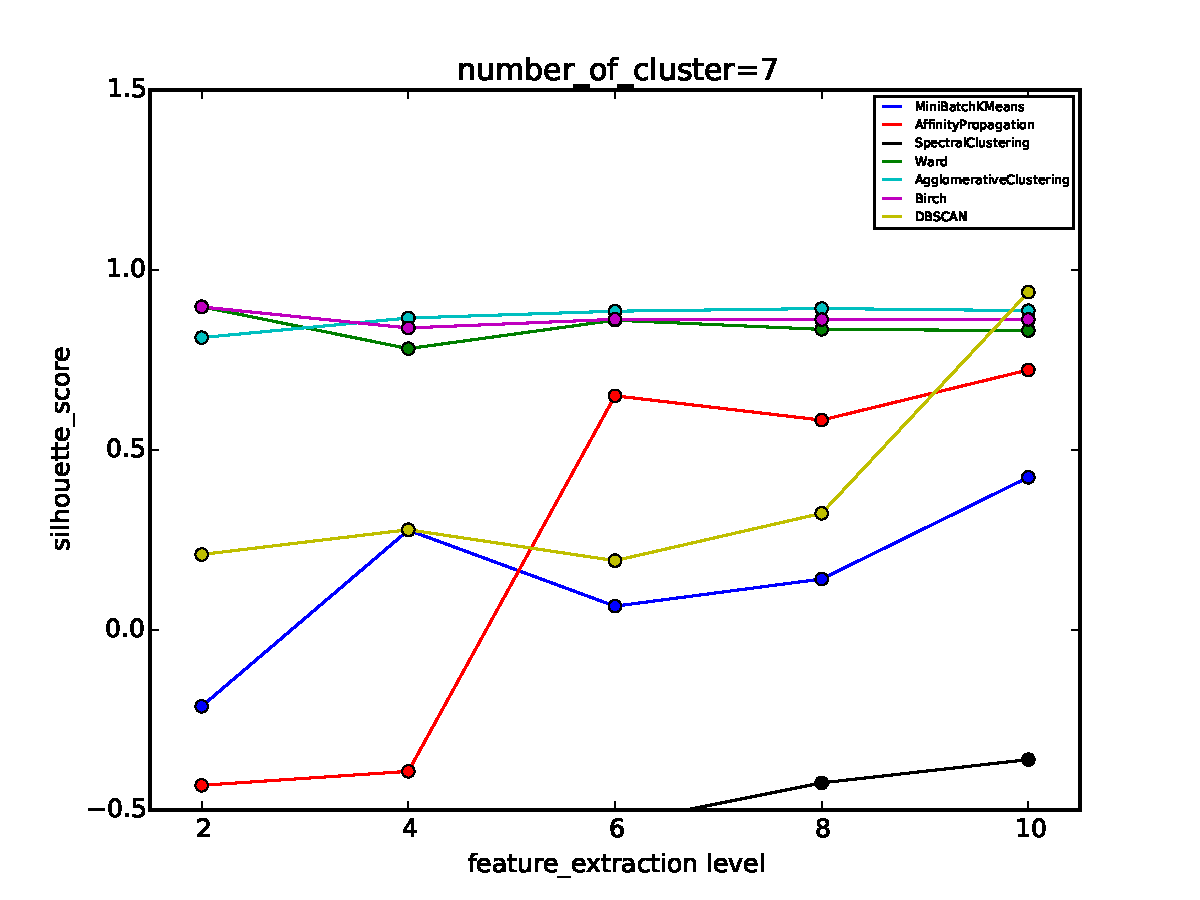
\includegraphics[width=0.49\textwidth]{../earthquakedata/output_plot/silhouette_score_plot_per_level_(clusters=7).pdf}}
\subfigure[Eight clusters]{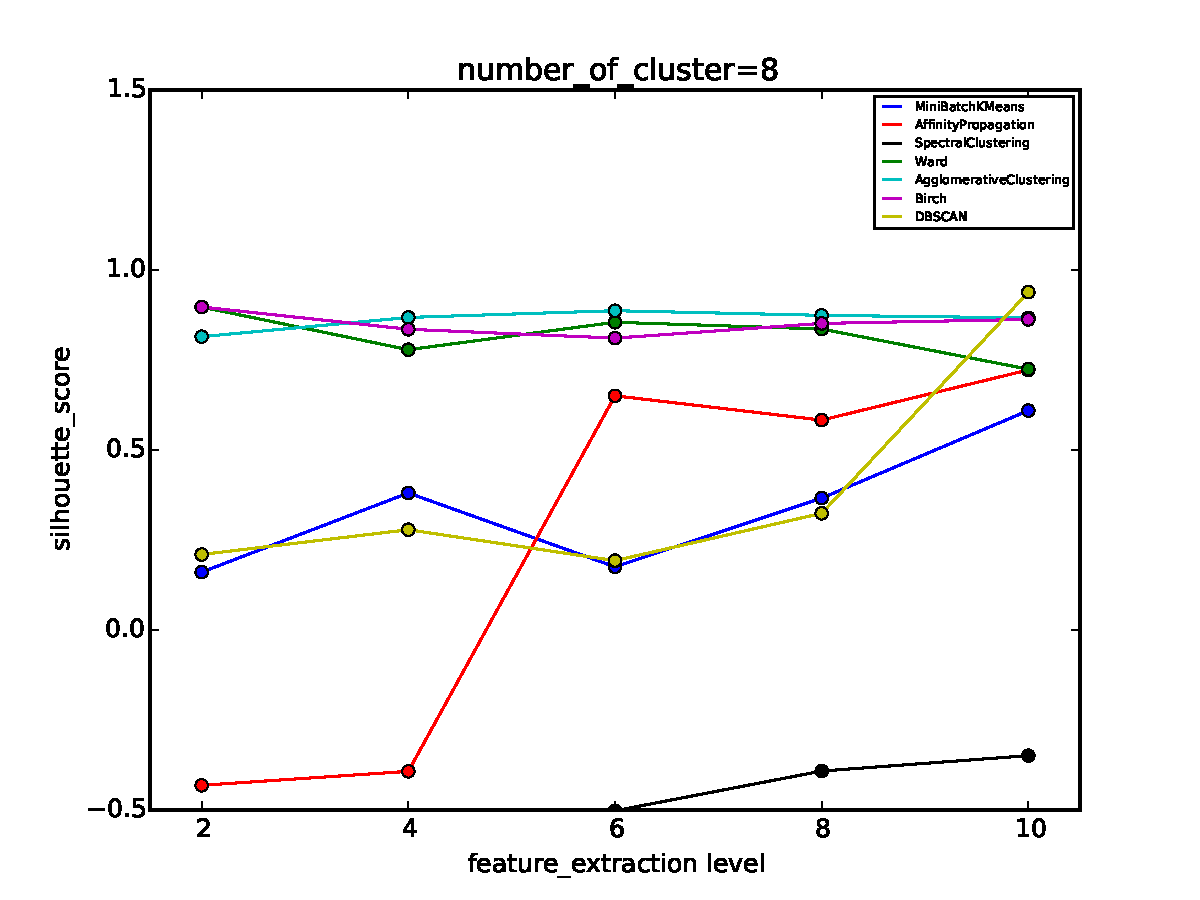
\includegraphics[width=0.49\textwidth]{../earthquakedata/output_plot/silhouette_score_plot_per_level_(clusters=8).pdf}}
\subfigure[Nine clusters]{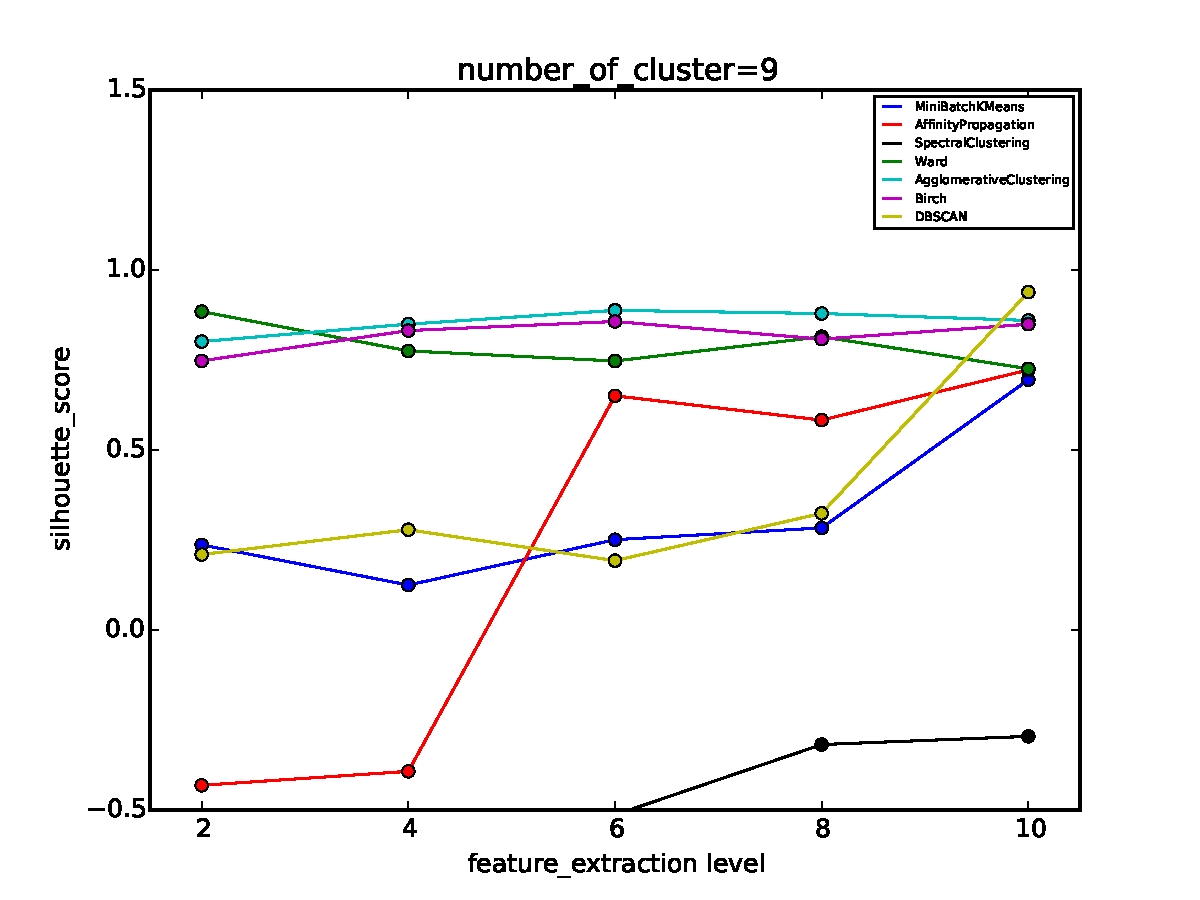
\includegraphics[width=0.49\textwidth]{../earthquakedata/output_plot/silhouette_score_plot_per_level_(clusters=9).pdf}}
\caption{Silhouette coefficient for various clustering levels on earthquake frequency dataset.} \label{silhouette_score_eq}
\end{figure}


\section{Examining Earthquake Data in more Detail}
\subsection{Objectives and Data Details}

The objective in examining earthquake data is two-fold: further investigate  the usefullness of Clustering Time Series using Wavlet decomposition for evaluating Earthquake data; and determine if there is a relation between earthquake occurrences and fracking.


Fracking is the process whereby a "mixture of water and chemical additives are pumped down the well at high pressure. This creates fractures in the rock, and a proppant such as sand is injected to keep the fracture open. This allows the natural gas to flow to the well and up to the surface"\cite{WFUS1}. 
"According to the Department of Energy (DOE), as of 2013 at least two million oil and gas wells in the US have been hydraulically fractured, and that of new wells being drilled, up to 95\% are hydraulically fractured" \cite{WFUS1}.
One source estimated that the average well depth is 7700 feet \cite{HSW1}.

Earthquake data details:
\begin{itemize}
\item The data was taken from http://earthquake.usgs.gov/data/
\item All data identified as type=earthquake  was collected for 2010-2014. The location of te earthquake was provied in longitude and latitude. The location was  categorized according to UTM zome location (Universal Transverse Mercator which represents all locations on Earth, excluding the Polar Regions inside a grid map of the Earth.)
\item For reviewing this data, it is important to note "magnitude 3 or lower earthquakes are mostly almost imperceptible or weak" \cite{WE1}.
\item The data includes  ~500 questionable records for 2013 and 2014. These records have a negative magnitude value. Since these records were extracted from a government site, and until 2013 the magnitude values had been positive, this author chooses to keep these values and consider the possibility that negative magnitude might be an indication of geographic condition rather than a data error.  I.E. given more of an experiential than a technical knowledge of earthquakes, perhaps a negative magnitude is viable.  Also these records represented less than 0.0056% of the data for 2013 or 2014.
\item  Converting Earthquake data to Time Series data involved creating an entry for each date within the years 2010-2014 for each UTM.  If there were no earthquakes on a specific date for the specific UTM, then the value was 0. If there were earthquake(s) for a specific date and specific UTM then the record contains the data, the UTM zone, the number of earthquakes, and a pair of values for each earthquake.  The value pair is the earthquake magnitude and depth.

\end{itemize}

\subsection{Earthquake Data Review}

Figure \ref{quakeboxplot} shows the box plots for the global and the USA earthquake magnitude for 2010 to 2014.  For both Global and USA, notice that the magnitude median is approximately 4 and the second and third percentiles (representing the percentage of data between 25\% and 75\%) is between 3 and 4.5.
For 2013 and 2014, the magnitude median is approximately 1.5 and the percentage of data between 25\% and 75\% is between 1 and 2.25.  This is a significant change from 2010 to 2012. 
Adjacent to the Global boxplot is a histogram showing the number of earthquakes for each year. There is a significant increase for 2013 and 2014 in comparison to 2010 to 2012.
I.e. There is a  ~390% increase in 2013 versus 2010, and a  ~500% increase in 2014 versus 2010. This suggests that as the number of earthquakes increased the increased earthquakes were of a lower magnitude.

\begin{figure}
\begin{center}
\subfigure[Global Earthquake Summary]{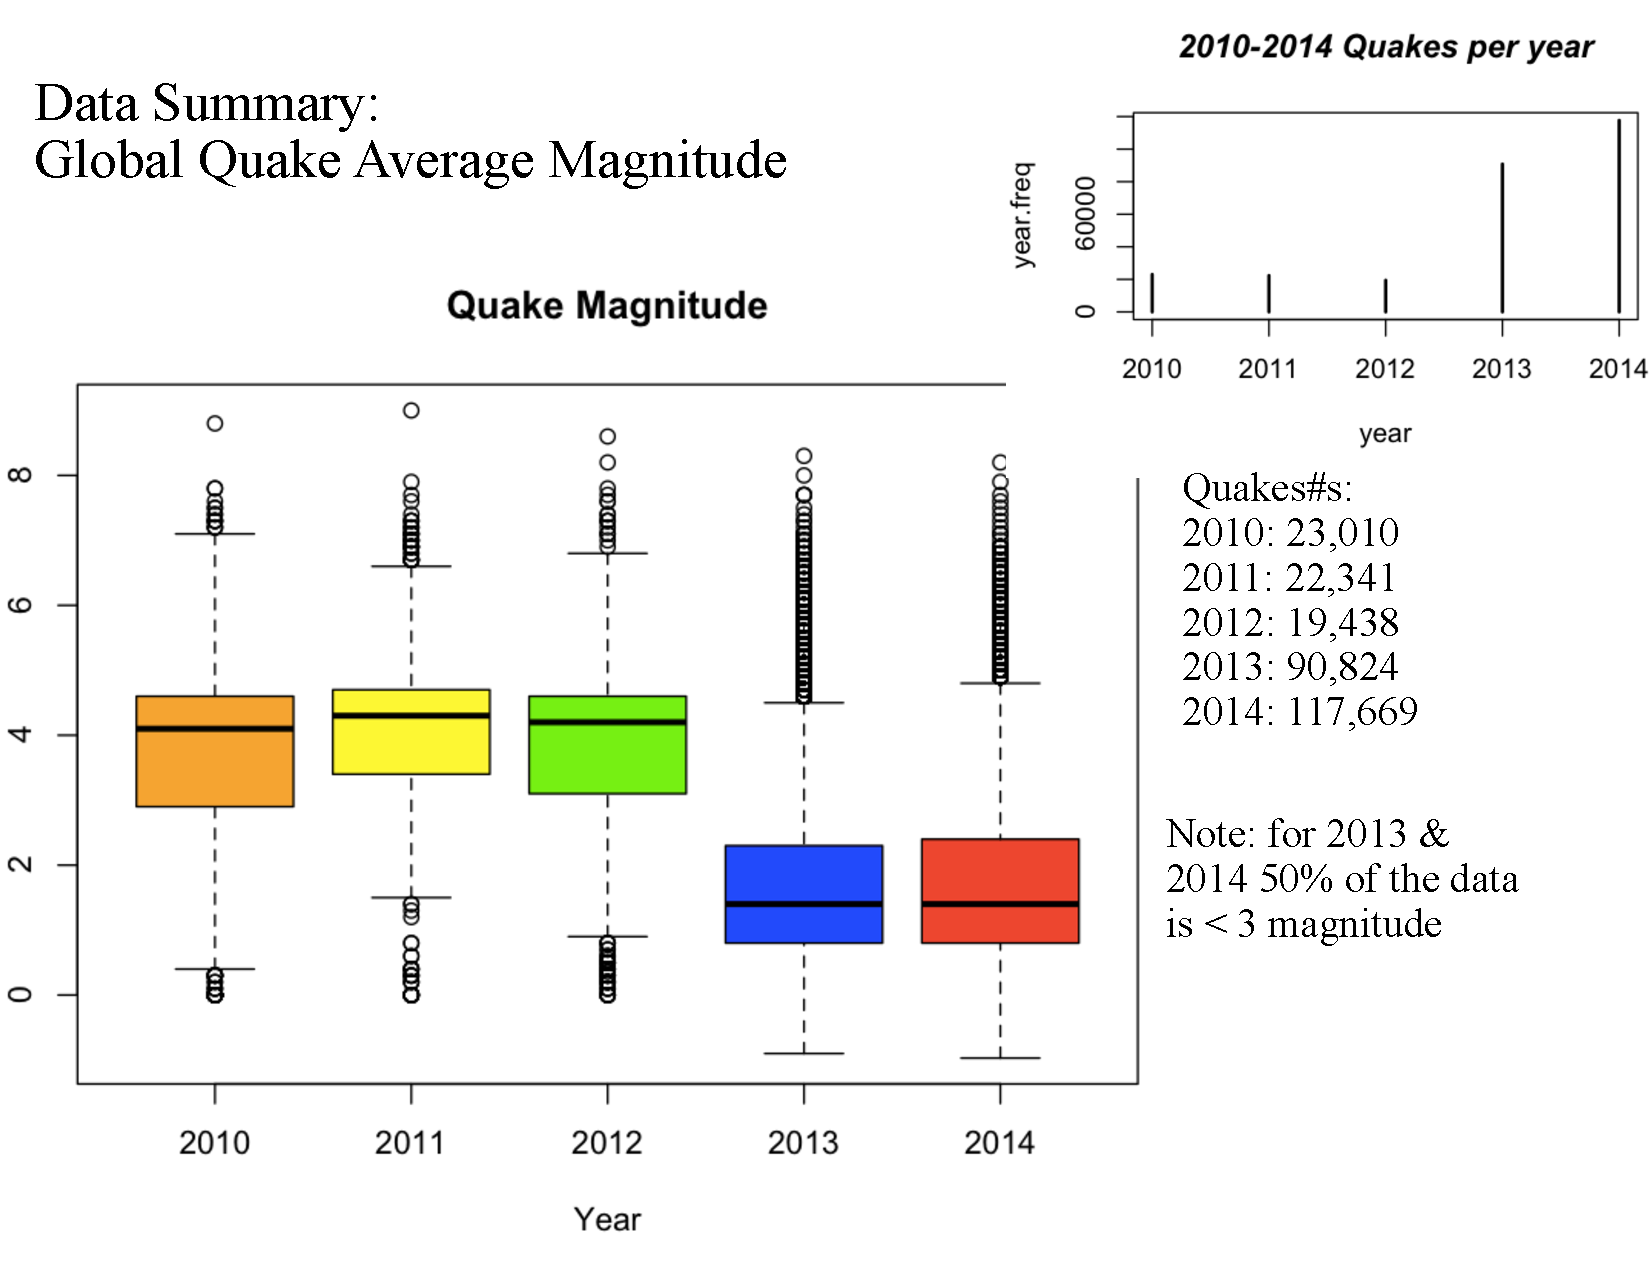
\includegraphics[width=0.49\textwidth]{../earthquake-analysis/global-quake-summary.pdf}}
\subfigure[USA Earthquake Summary]{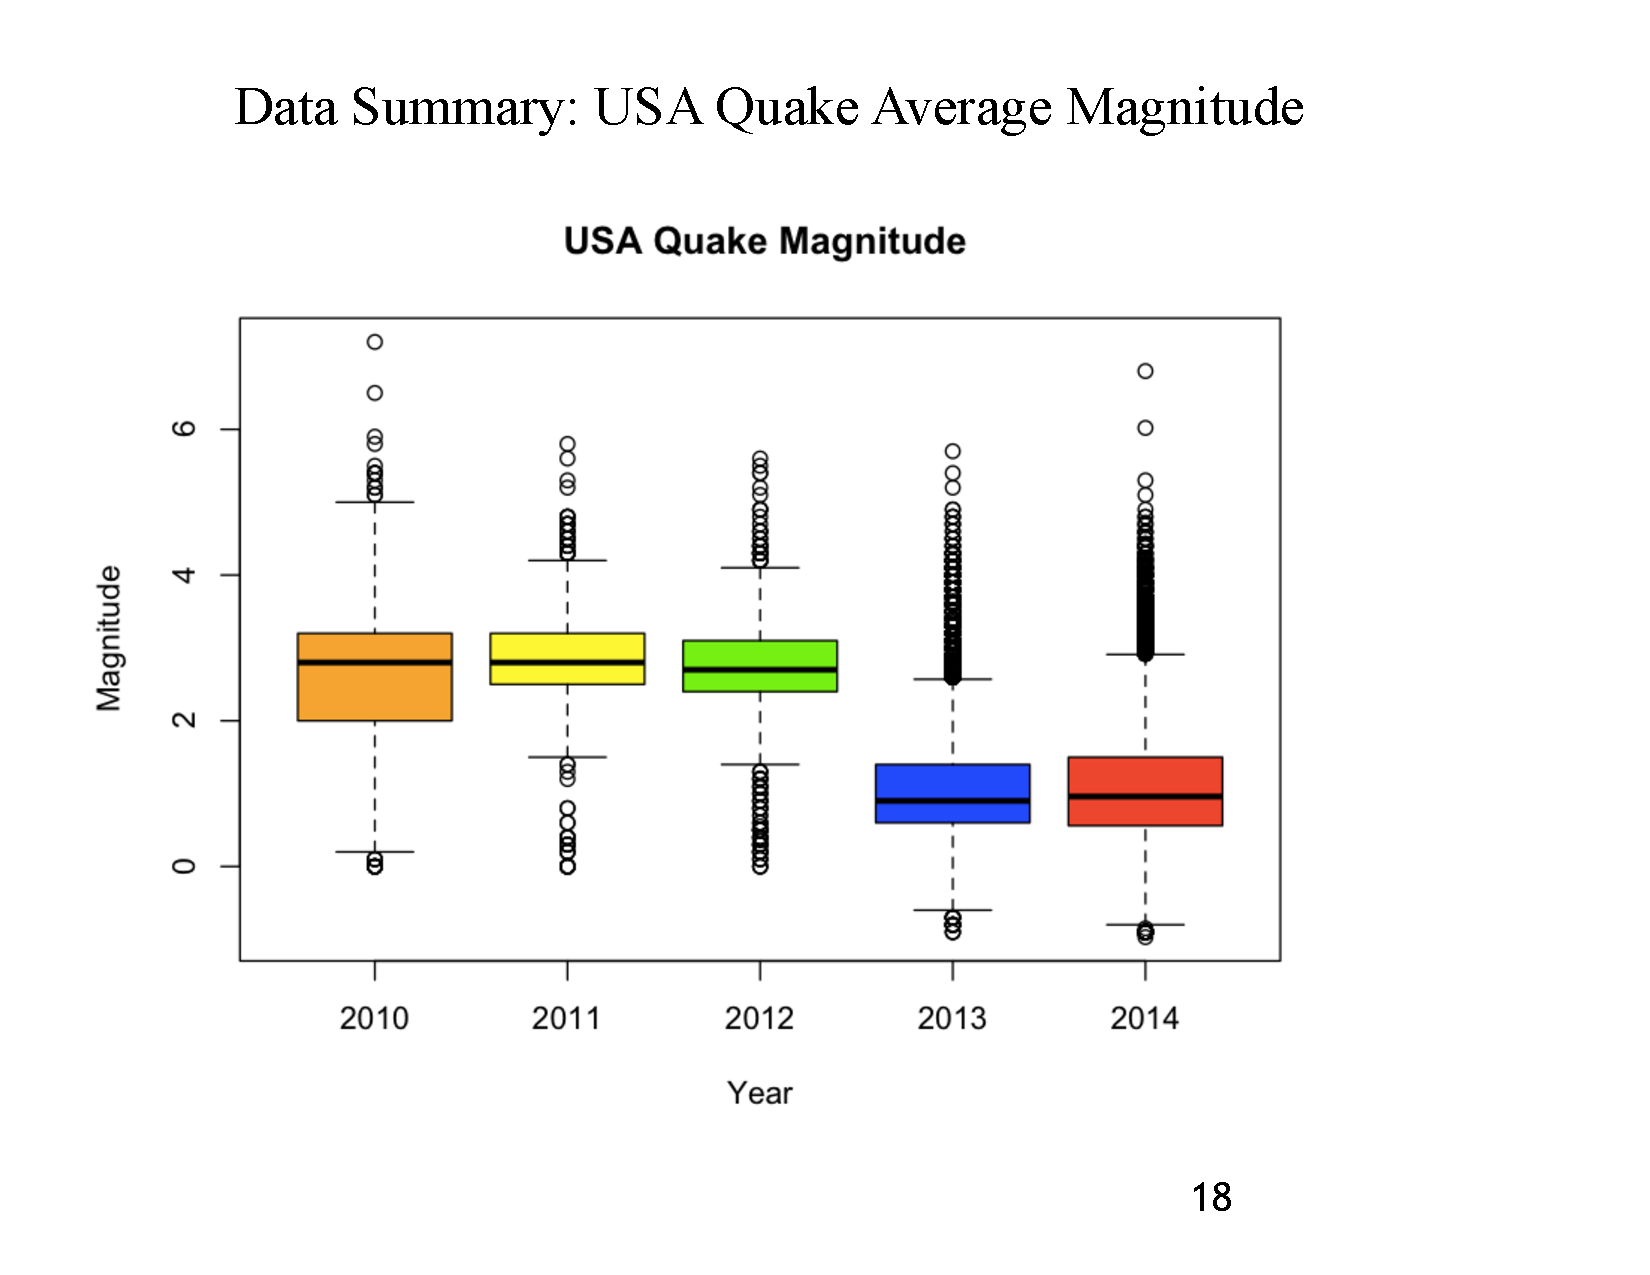
\includegraphics[width=0.49\textwidth]{../earthquake-analysis/usa-quakes-summary.pdf}}
\caption{Global and USA Earthquake Magnitude boxplot.} \label{quakeboxplot}
\end{center}
\end{figure}

Figure \ref{quakesbyutm} show the frequency of earthquakes for each MTU zone by year.
Notice the zones with the highest frequency are 10S, 11S, 14S, 10T, 11T, 12T. By referring to the USA map of UTM zones, 10S and 11S are California, and 14S is Texas and Oaklahoma.
The MTU zones 10T, 11T, and 13T are Washington, Oregon, Idaho, Montana, and Wyoming.

This author realizes that an more extensive study is required to identify the frequency of fracking in each state. 
At this tme, the author can provide a discussion for the increase in fracking in California involving specific counties cite{QF1}, plus the report of increased earthquake activites in Texas and Oaklahoma some people have attributed to fracking cite{QF2}.

\begin{figure}
\begin{center}
\subfigure[USA Earthquake frequency for UTM zone, by year]{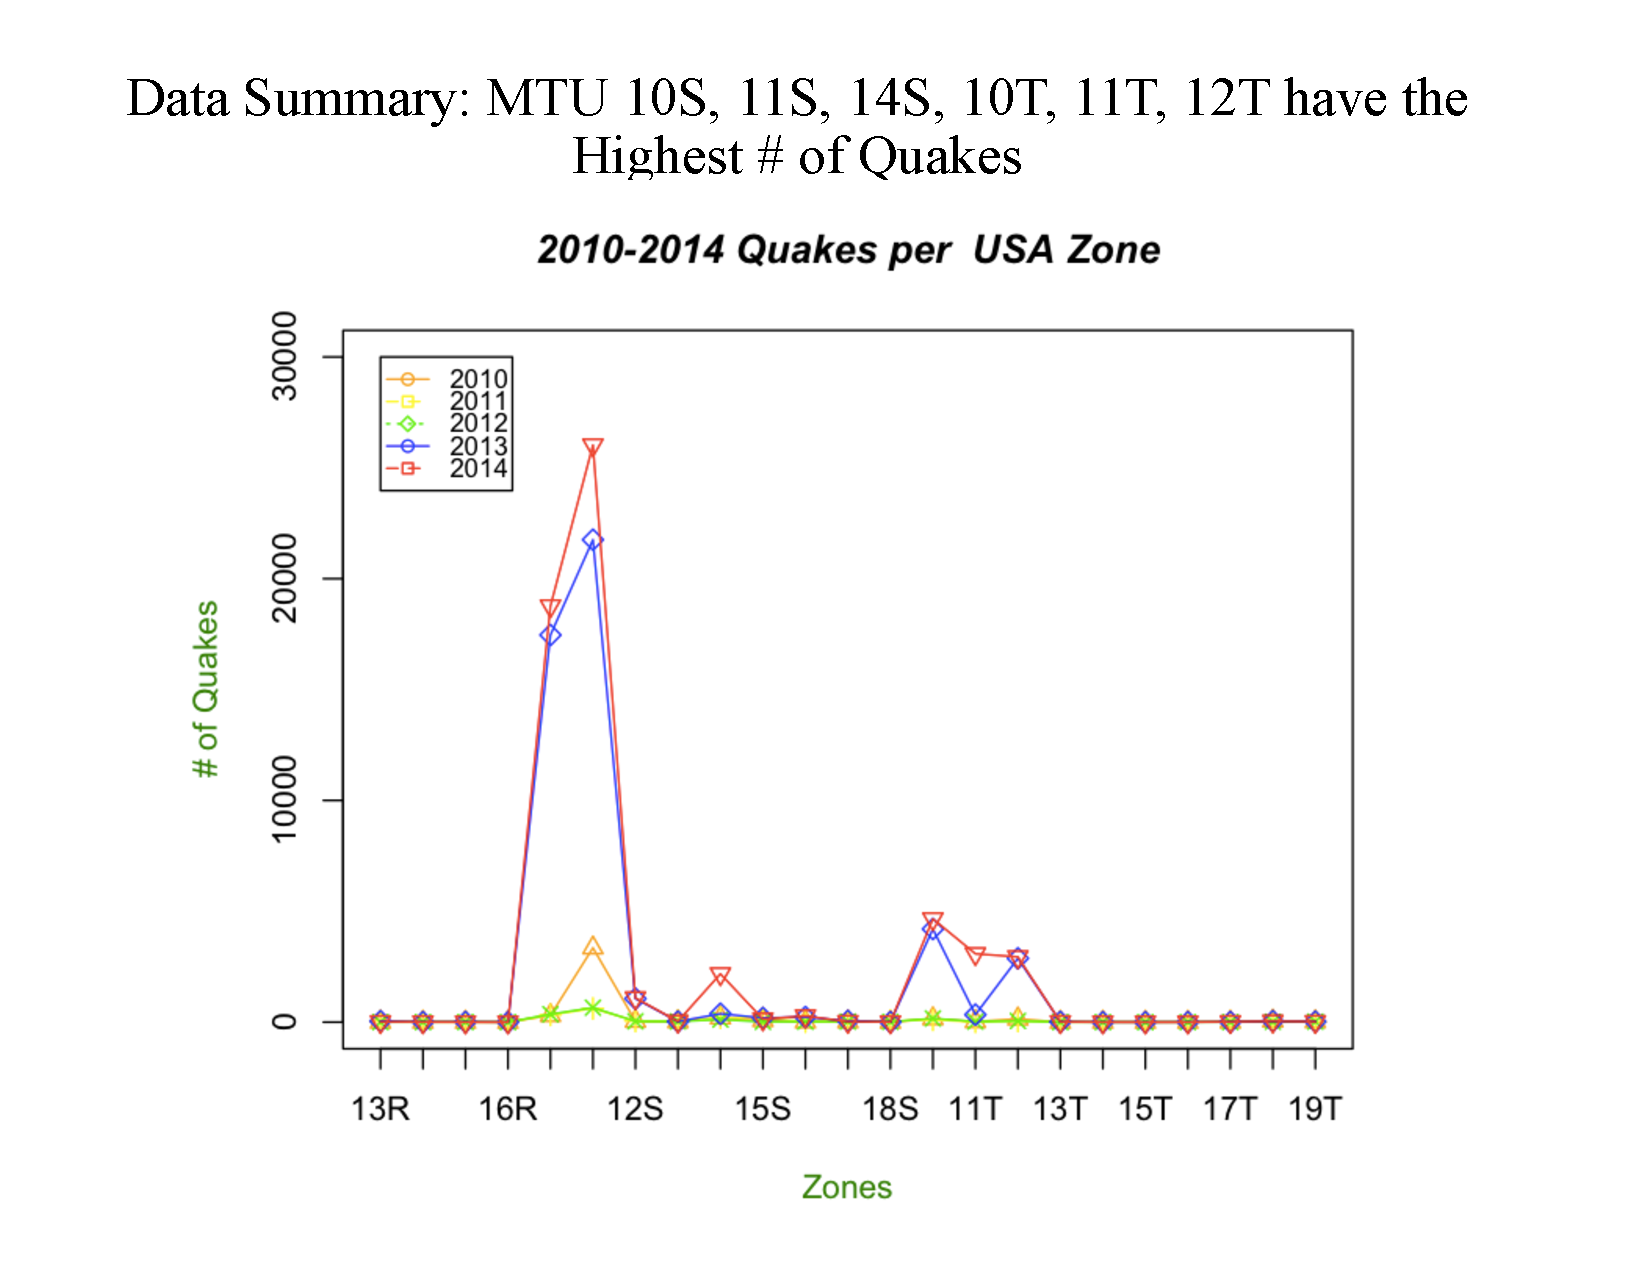
\includegraphics[width=0.49\textwidth]{../earthquake-analysis/usa-quakes-mtu-summary.pdf}}
\subfigure[USA map of UTM zones]{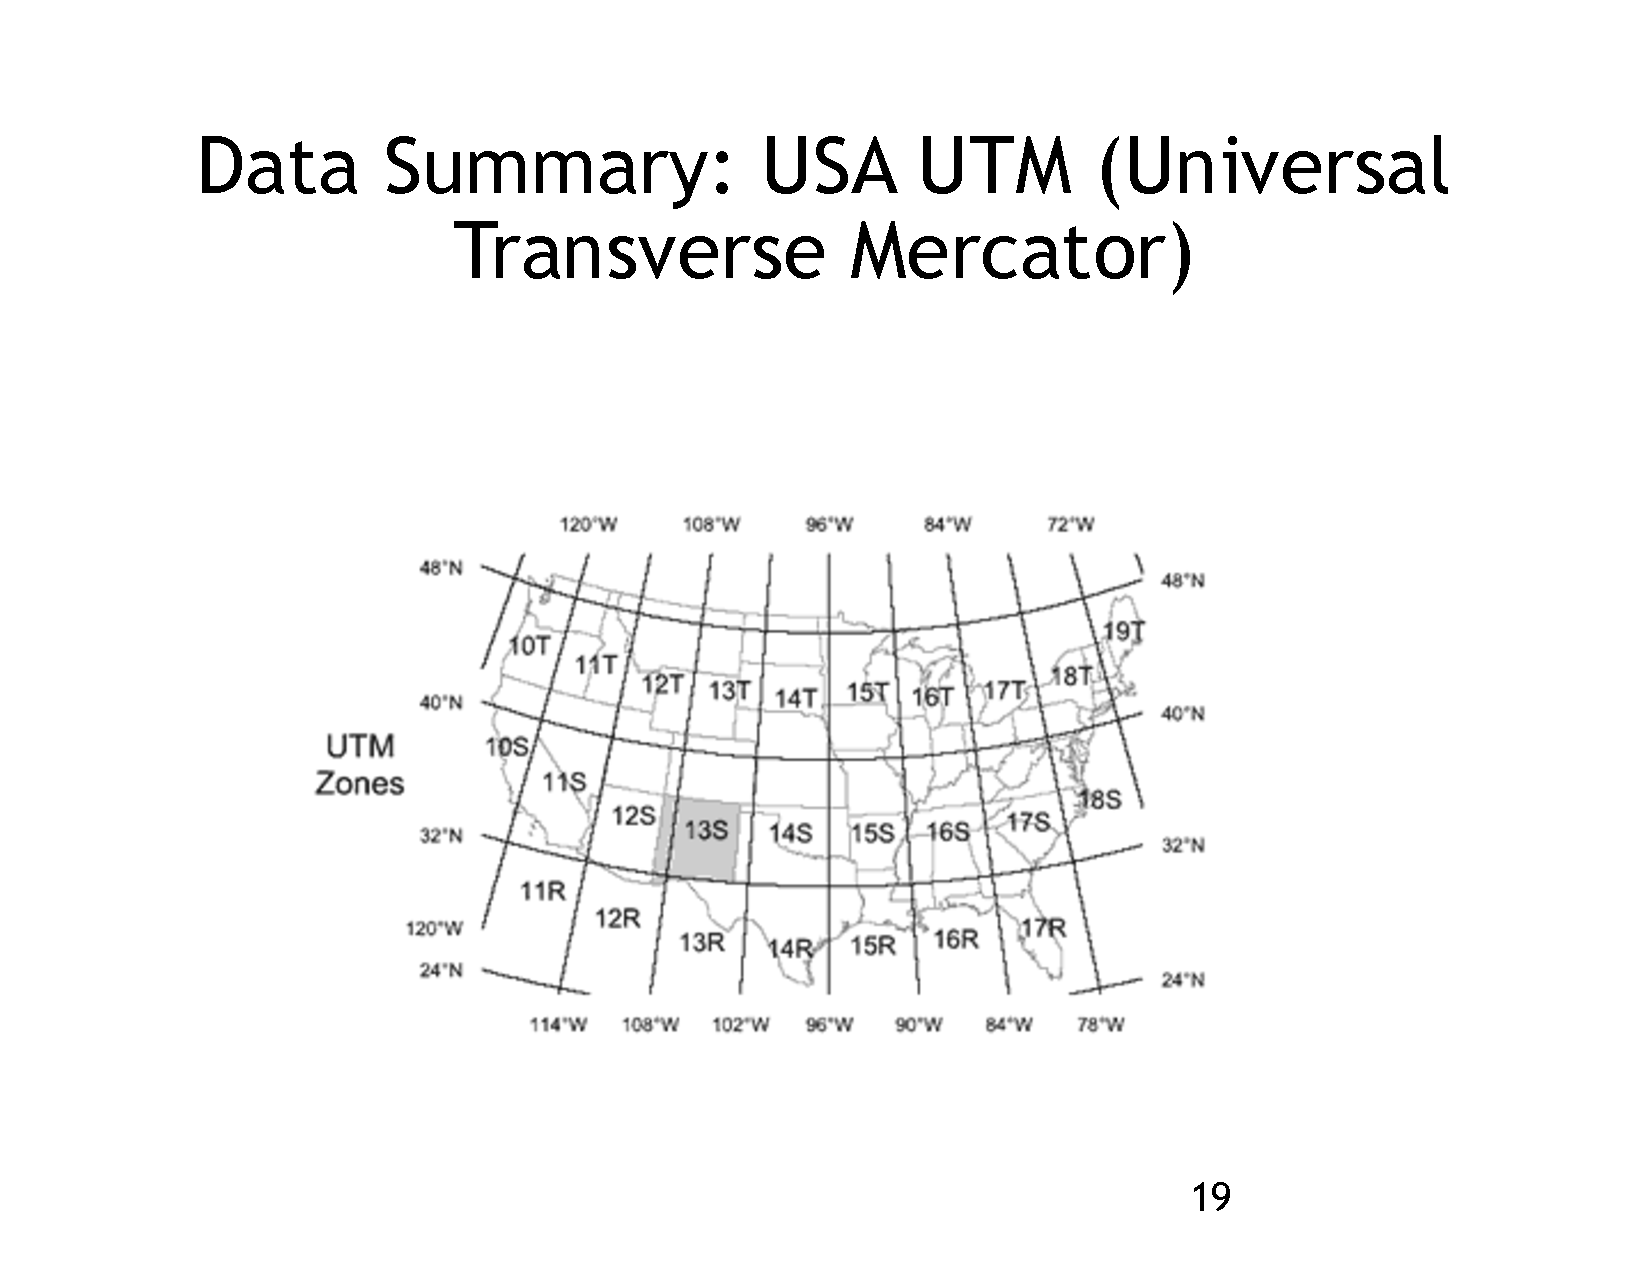
\includegraphics[width=0.49\textwidth]{../earthquake-analysis/usa-utm.pdf}}
\caption{USA Earthquake frequency by UTM zone and year,  with USA map.} \label{quakesbyutm}
\end{center}
\end{figure}


\begin{figure}
\begin{center}
\subfigure[Clustering USA quakes for 2010 and 2014]{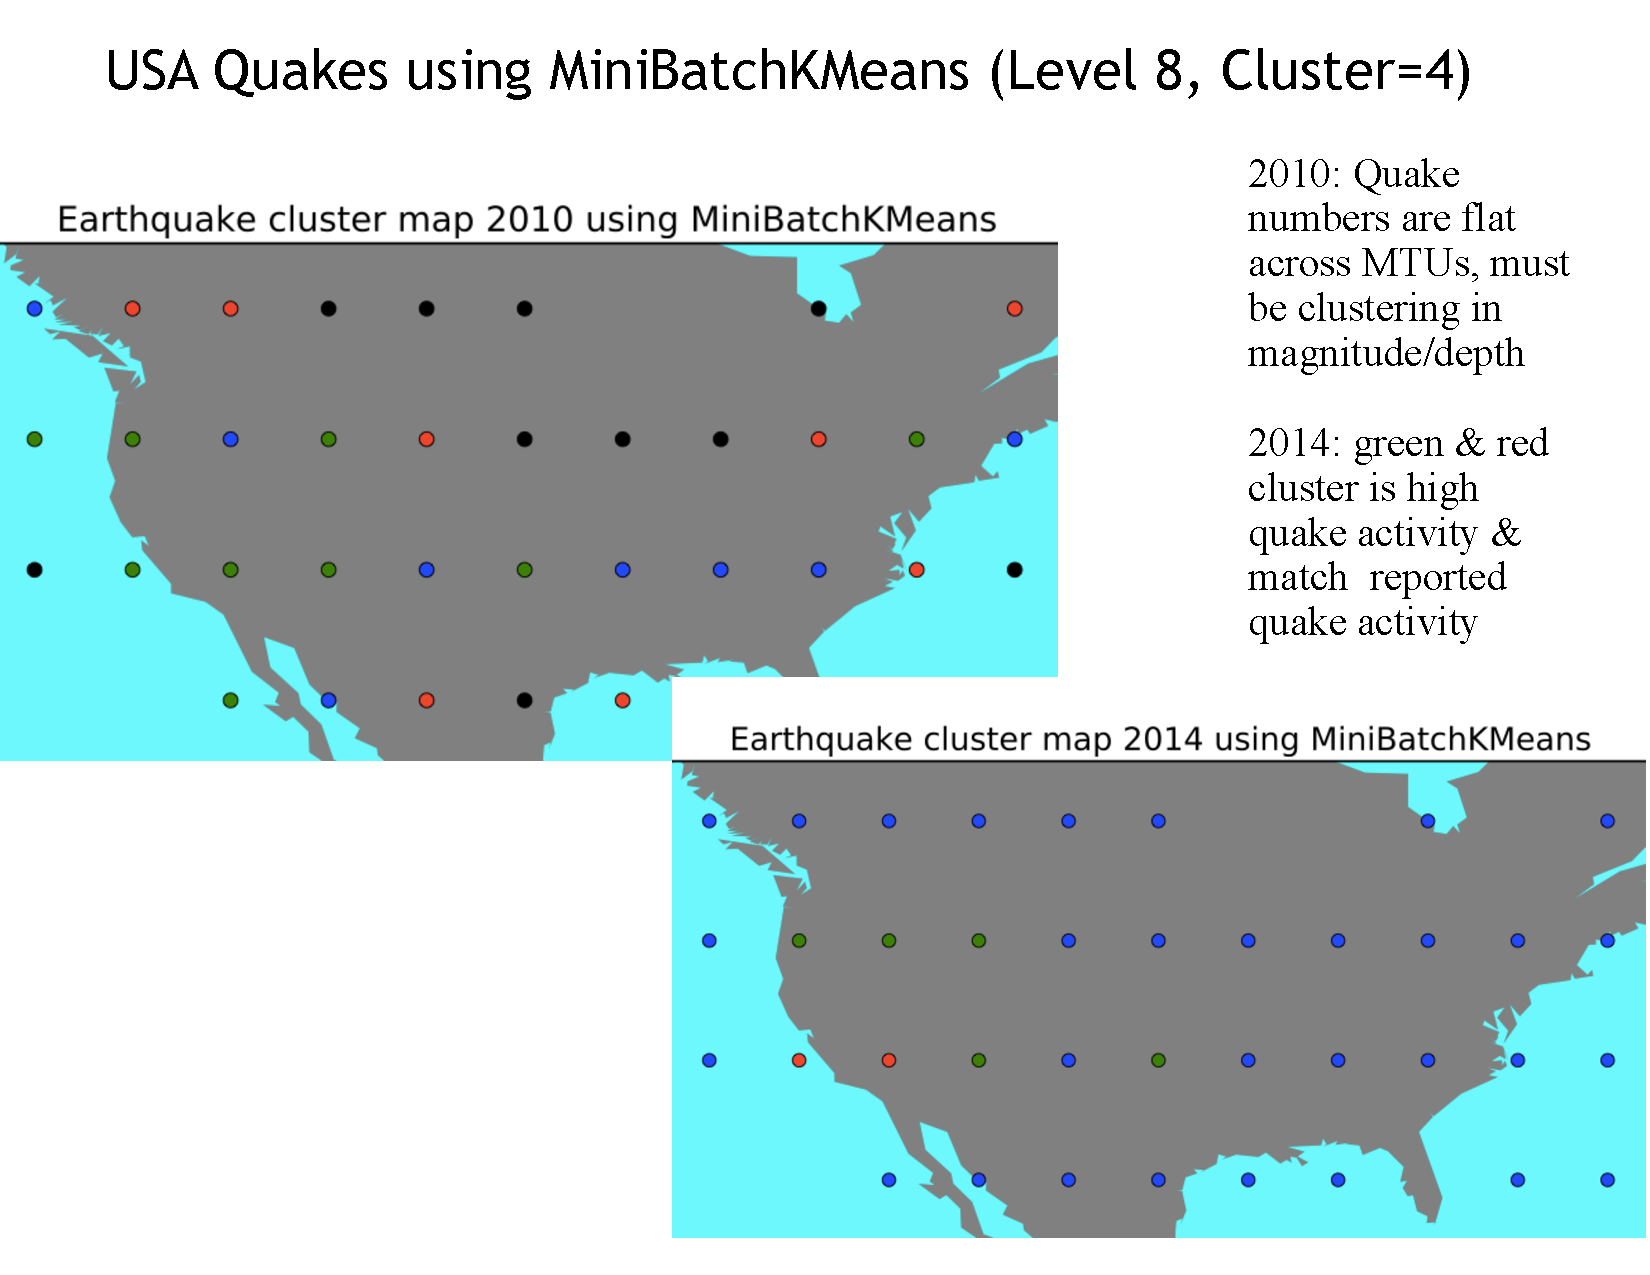
\includegraphics[width=0.49\textwidth]{../earthquake-analysis/usa-quakes-cluster.pdf}}
\caption{USA Earthquake Cluster using Kmeans.} \label{quakecluster}
\end{center}
\end{figure}

Figure \ref{quakecluster} shows clustering of USA Earthquakes for 2010 and 2014.  The 2010 cluster does not seem to display any relationship between earthquake frequency and color of the cluster.
Although there is multicolor points indicating that Earthquake characteristics did cluster.  Recall that magnitude and depth are also clusteriig values.  Perhaps magnitude and depth played a large role in assigning cluster for 2010.
For year 2014, one can speculate that the MTU zone color is related to earthquake frequency.  For example the red cluster is the MTU zones 10S and 11S, which is Californis and part of Nevada.
The green cluster is the MTU zones 14S, 10T, 11T, and 12T which had high earthquake frequency.
\subsection{Earthquake Conclusions}

\begin{itemize}
\item Earthquake data can be examined using Time Series with Wavelet Transformations.
\item There appears to be a relationship between Fracking and increased Earthquake frequency.
\item The presence of Fracking in a geography appears to be linked to Earthquakes of less than or equal to  magnitude 3. This does not exclude the possibility that Fracking is linked with Earthquakes of  greater than 3 magnitude.
\end{itemize}


\section{Conclusions}

This project investigated the use of wavelet transformations as a feature extraction mechanism for the clustering of time series. A framework to evaluate the concept was developed and tested on three different time series data sets: closing prices for stocks, currency exchange rates, and earthquake data.

The results of the experimental evaluation suggest that {\em both} a qualitative assessment as well as the evaluation of a number of measurements, such as the silhouette coefficient, are necessary to understand the data set and the particular combination of parameters for which a clustering algorithm offers the best performance. A premise of the project was that wavelet transformation as a feature extraction mechanism could potentially result in better clusterings. However, the results show that the silhouette coefficient for stock price data is relatively less sensitive to the degree of dimensionality reduction provided by the transformation (clustering level) than the coefficient for earthquake data. The result shows that we need to identify important sets of parameters for each data set. As part of a process to improve the quality of the clusterings, complementary performance measurements would need to be included in the evaluation.



\appendix
\section*{Appendix A: Stock symbols}
\label{AppA}

YHOO, GOOGL, AAPL, MSFT, BIDU, IBM, EBAY, ORCL, CSCO, SAP, VZ, T, CMCSA, AMX, QCOM, NOK, AMZN, WMT, COST, TGT, CVX, TOT, BP, XOM, E, COP, APA, GS, MS, BK, CS, SMFG, DB, RY, CS, BCS, SAN, BNPQY, NKE, DECK, PCLN, EMC, INTC, AMD, NVDA, TXN, BRCM, ADI, WFM, TFM, INFN, CIEN, CSC, TMO, BSX, TIVO, DISH, SATS, LORL, ORAN, IMASF, IRDM, HRS, GD, BA, LMT, NOC, RTN, TXT, ERJ, UTX, SPR, BDRBF, AAL, DAL, HA, UAL, LUV, JBLU, ALGT, RJET, RCL, CCL, DIS, CBS, FOXA, QVCA, DWA, VIAB, TM, TWX, DISCA, SNI, MSG, PG, ENR, HRG, SPB, KMB, TSLA.

\section*{Appendix B: Earthquake UTM zones}
\label{AppB}

C5-6, C8, C58, D1-2, D16, D41, D49, D53, D58, D59, D60, E10, E19, E20-29, E3-7, E38, E55-59, F10-18, F2, F20-36, F42-43, F47-49, F5, F50-58, F6-9, F60, G12-19, G21, G27-29, G36-38, G43-48, G51-52, G55-56, G58-60, H1, H11-15, H18-20, H24, H28-29, H34, H37-40, H43-44, H48-49, H51, H53-56, H59-60, J1-3,  J7, J11-12, J17-20, J28-29, J33-37, J40-45, J49, J51-54, J56, J58-60, K1-2,  K6, K11-12, K18-20, K23-24, K28-29, K33, K35-39, K41-42, K44-45, K47, K49-53, K55, K57-60, L1-3, L9, L12-15, L1720, L22, L28-30, L33-39, L41-42, L45-53, L55-60,  M10, M12-15, M17-20, M22, M25-30, M32, M34-37, M39, M42-57, N10, N13-19, N22, N24-26, N28, N34-37, N40-47, N49-53, N55, P12-24, P26-29, P37-40, P45-56, Q4-5, Q10-21, Q23, Q26, Q28-29, Q31, Q37-39, Q41-52, Q54-55, R11-16, R18-20, R23-24, R27, R29, R35-36, R38-49, R5, R8, R50-60, S9-20, S24-55,  T9-39, T41-57, U1-14, U17, U19-20, U22, U25-26, U29-34, U36, U41, U43-52, U54-60, V1-8, V10, V20-21, V23, V25-27, V30-33, V35, V40-42, V47, V49-52, V55-60, V7-9, W1-10, W15-16, W18-22, W25, W27-34, W41, W51-52, W54-55, W59, X5, X9-12, X14-18, X21, X25-27, X29-31, X33, X41, X49-53

\begin{thebibliography}{1}

\bibitem{BGRS99} K. Beyen, J. Goldstein, R. Ramakrishnan, and U. Shaft. When is nearest neighbor meaningful? In {\em Proceedings of the 7th International Conference on Database Theory}, pp. 217-235, 1999.

\bibitem{ZHZL06} H. Zhang, T. B. Ho, Y. Zhang, M.-S. Lin. Unsupervised Feature Extraction for Time Series Clustering Using Orthogonal Wavelet Transform. In {\em Informatica}, Volume 30, pp. 305-319, 2006.

\bibitem{C92} C. K. Chui. {\em An Introduction to Wavelets.} Academic Press, San Diego, 1992.

\bibitem{D92} I. Daubechies. Ten Lectures on Wavelets. {\em SIAM}, Philadelphia, PA, 1992.

\bibitem{MAFG82} J. Morlet, G. Arens, E. Fourgeau and D. Giard. Wave propagation and sampling theory, Part 1: Complex  signal land scattering in multilayer media. {\em Journal of Geophysics,} 47:203-221, 1982.

\bibitem{CGT89} J. M. Combes, A. Grossman and P. Tchamitchian, editors. {\em Wavelets, Time-Frequency Methods and Phase Space.} Springer-Verlag, Berlin 1989.

\bibitem{D88} I. Daubechies. Orthonormal bases of compactly supported wavelets. {\em Communications on Pure and Applied Mathematics,} 41:909-996, 1988.

\bibitem{BGG98} C. Sidney Burrus, R. A. Gopinath, and H. Guo, {\em Introduction to Wavelets and Wavelet Transforms: A Primer,} Prentice Hall, NJ 1998.

\bibitem{TSK05} P.-N. Tan, M. Steinbach, and V. Kumar. {\em Introduction to Data Mining,} Pearson, First Edition, 2005.

\bibitem{FRED15} Federal Reserve Economic Data (FRED) service, {\em https://research.stlouisfed.org/fred2/}. Accessed: May 27th 2015.

\bibitem{HSW1} How Stuff Works {\em http://science.howstuffworks.com/environmental/energy/hydraulic-fracking1.htm/}.

\bibitem{SKL15} SciKit Learn {\em http://scikit-learn.org/stable/}. Accessed: May 27th 2015.

\bibitem{WE1} Wikipedia Earthquakes {\em http://en.wikipedia.org/Earthquake/}.

\bibitem{WFUS1} Wikipedia Fracking {\em http://en.wikipedia.org/Hydraulic\_fracturing\_in\_the\_United\_States/}.

\bibitem{WTP15} Wikipedia Tectonics {\em http://en.wikipedia.org/Plate\_tectonics/}.

\bibitem{QF1} California and Fracking {\em http://www.biologicaldiversity.org/campaigns/california\_fracking/faq.html/}.

\bibitem{QF2} Texas and Oaklahoma have Fracking concerns {\em http://www.natlawreview.com/article/oklahoma-joins-texas-preventing-local-fracking-bans/}.

\bibitem{QF3} Man made Earthquakes {\em	http://www.usgs.gov/blogs/features/usgs\_top\_story/man-made-earthquakes/}.

\end{thebibliography}

\end{document}
